\documentclass[12pt,a4paper,notitlepage]{article}
\usepackage[utf8]{inputenc}
\usepackage[english]{babel}
\usepackage[T1]{fontenc}
\usepackage[backend=biber,
			style=authoryear-comp,
			isbn=false,
			doi=false,
			bibstyle=authoryear,
			natbib,
			]{biblatex}
\usepackage{eurosym}
\usepackage{enumitem}
\usepackage{url}
\usepackage{blindtext}
\usepackage{hyperref}
\usepackage{breakurl}
\usepackage{amsmath}
\usepackage{titling}
\usepackage{amsfonts}
\usepackage{amssymb}
\usepackage{pgfplots}
\usepackage{caption}
\usepackage{subcaption}
\usepackage{graphicx}
\usepackage{dcolumn}
\usepackage{tikz-3dplot}
\usepackage{subcaption}
\usepackage{float}
\usepackage{adjustbox}
\usepackage{multirow,rotating}
\usepackage[autostyle]{csquotes}
\usepackage[toc,page]{appendix}
\usepackage{lscape}
\usepackage{todonotes}
\usepackage{booktabs}
\usepackage{multirow}
\usepackage{bm}
\usepackage{eurosym}
\usepackage{pdflscape}

\addbibresource{Textmining.bib}

\begin{document}

\section{Introduction}

In Germany, the debate about the role of public media and their mission in a rapidly changing media world is a recurring theme. By shifting media content to the Internet, the dual system, which has been shaping the German television and radio landscape since the introduction of private broadcasting in the early 1980s, is facing a radical change. Since 2000, public broadcasting has expanded its range of services, particularly in the digital media sector. If the right to use digital media were to be withdrawn from the public media outlets, they would not only be deprived of the possibility of improved information provision. They also threatened to lose their competitiveness with commercial media. On the other hand, there is the concern of commercial providers who are registering an ever-increasing number of digital services financed by fees. They complain about a bias in competition caused by public media offering online text-content because of their fee financing. The advertising-financed business model of the media houses is based on the premise that users visit their websites in order to achieve high advertising revenues.

The fundamental question in this debate is whether the offer of public news on the internet is justified. They should only occur where there are clear deficits in private sector supply. A frequently cited argument is that only the public media make it possible to provide information that is free of self-interest. Due to their public mandate and financing, they can afford what private providers cannot or only to a limited extent because of their economic dependency: a journalistic and editorial self-observation of society in the public interest. Due to their constitutional determination, they are obliged to the diversity and representation of the political and social spectrum of opinion in its entire breadth, including minority positions.

On the basis of these justifications, this paper examines whether public media offer different content than private providers. In other words, whether socially desired content that meets the (social) needs of society and is therefore politically desirable is not provided by the market of private news, but by public providers. In order to examine this, the online news content of public media is compared with the supply of private news providers.

We use a data set of German online news articles about domestic politics to examine the differences in news content between public and private news provides. Your dataset contains articles dated from 01.06.2017 to 31.12.2017\footnote{German federal elections took place on 24th of September 2017.} from seven German content providers to analyze news reports about german elections, where we allow prevalence of topics to evolve over time (before and after the elections) and vary across newswire services. We then estimate the effect of news wire source on both topical prevalence (topic distribution) and topical content (word-topic distribution). 

Mapping raw text to one or more topics, without having prior knowledge on what those topics are, translates to an unsupervised classification problem on natural language. Topic models generate low-dimensional representations of data and can uncover interesting latent structure in large text datasets. They are popular tools for automatically identifying prominent themes in text. Within topic models the Latent Dirichlet Allocation (LDA) is a widely used technique, where each document (article) is viewed as a mixture of topics (represented by the document-topic distribution) and each topic is a mixture of unique terms, represented by the topic-term distribution \citep{blei_latent_2003}. \citet{roberts_model_2016} extents the base idea of LDA by developing a structural topic model (STM) that allows to incorporate external variables that effect both topical content and topical prevalence. We use this approach to analyze online news about the german domestic politics, where we allow prevalence of topics to vary across newswire services. We then estimate the effect of topical prevalence (the posterior document-topic distribution) on the ownership (public or private).

The paper proceeds as follows: The next section (\ref{ch_onlinenews}) briefly explains the market for online news in Germany. We will examine the largest players on the market and use keyword analytics to investigate which providers are similar. Section \ref{ch_model} explains the generative process of the mixed membership model and the results of this process are presented in chapter \ref{ch_results}. Chapter \ref{ch_data} contains a description of the text data and how it was pre-processed in order to use it as input variable. Chapter \ref{ch_regression} describes how we regress the estimated probabilities of topic prevalence of a document on its metadata.

% ----------------------
% the online news market
% ----------------------
\section{The online news market}\label{ch_onlinenews}

The market for media content in Germany is characterized by the coexistence of public and private broadcasters. By shifting media content to the Internet, the dual system, which has been shaping the German television and radio landscape since the introduction of private broadcasting in the early 1980s, is facing a radical change. Since 2000, public broadcasting has expanded its range of services, particularly in the digital media sector. In 2017, 22 own websites and 100 apps were operated by public broadcasters on which they offer their content. As a result, public broadcasting no longer only competes with private television and radio stations, but also enters the market for online news. In the following, we will briefly discuss the characteristics of the market for online news. 

Private media outlets naturally appear as two-sided platforms, that allow interaction between two categories of consumers: audiences and advertisers. As the demand on both consumer-sides are linked via indirect network externalities, the market in which media outlets operate are referred to as two-sided or multi-sided markets. The theoretical literature on two-sided markets originates from the analysis of credit card markets \citep{rochet_platform_2003} and was later transferred to the concept of other industries, such as dating agencies, real estate agents, and internet “business-to-business” websites \citep{caillaud_chicken_2003}. The basic concept of two-sided markets was already discussed decades ago in several economic studies, especially on media markets \citep{corden_maximisation_1952}, \citep{gustafsson_circulation_1978}, \citep{blair_pricing_1993}. However, comprehensive analyses have only been carried out in the last ten years, starting with the works of \citet{rochet_platform_2003}, \citet{evans_empirical_2003} and \citet{armstrong_competition_2006}.

Advertising-supported media such as online newspapers are typical examples of two-sided markets where the newspaper can be conceived as platforms that allow interaction between audiences ("eyeballs") and advertisers. The newspaper creates (or buys) content to attract viewers which in turn attract advertisers who pay for readers' attention.\cite{evans_industrial_2005} The size and characteristics of the audience has a positive effect on the advertisers' willingness to pay, as advertisements are typically sold based on cost per viewer, often expressed in terms of the cost of reaching a thousand viewers (CPM). Advertising can also have an effect on the recipients, which can be both negative and positive, depending on the quality of the advertising. Depending on the strength of the indirect network effects, private publisher maximize their revenue by balancing the demand from advertisers and subscribers using different business models \citep{evans_economics_2008}. Many traditional newspapers follow the subscription/advertising model, where the publisher charges both market sides: The audience pays a fee to obtain access to the content, and advertisers pay to obtain access to the viewers. Many online news agencies provide part of their editorial content for free and hide another, more exclusive part behind a paywall. However, since the Internet has considerably simplified the possibilities for obtaining information and thus reduced the marginal utility of content, such a business model can only be efficient if the content is very exclusive. As a result, many publishers rely on a free-media model, in which the publishers do not charge viewers for access to the media at all, in order to attract as many eyeballs as possible to their platform, and thus exploit the indirect network effects on the advertising site. In fact, most advertising-financed online magazines earn their gross margin from advertising.\cite{evans_industrial_2005} In order to maximize their profits, these companies have an interest in attracting as many readers as possible. In addition to the quantity of the audience, the demographic characteristics of recipients also have an influence on the willingness to pay on the advertiser site. Online advertising makes it possible to target ads to particular consumers in real time.
 
The two-sided market structure of the private news markets results in news platforms striving to choose their content in such a way that its reach is as large as possible in order to maximize profits from advertising revenues. \citep{steiner_program_1952} concluded, that profit-maximizing media owners may choose to offer the same content, i.e. content aligned with the tastes of the majority. \citep{gabszewicz_press_2001} study the problem of diversity of the political content of newspapers. They find that the maximum differentiation only prevails if the readers sufficiently value the political differentiation between the newspapers the advertising market is small enough. On the other hand, advertising may also have a positive impact on the media, as it enables publishers to report independently of political parties. \citet{ellman_what_2009} found that advertising increases the intensity of competition for readers and therefore raises accuracy of media coverage. 

Given the crucial role of the media in shaping opinion and promoting democracy, pluralism of opinion and accuracy of information is a major concern of public authorities. Public broadcasting in Germany originated in the post-war period and has always had the task of providing the entire population with independent media. This media offer is intended to guarantee diversity of opinion within the media landscape and to be economically and politically independent. The former is given by the fact that the public media are financed by compulsory fees. To take into account the distinct nature of digital media, the Interstate Broadcasting Agreement (Rundfunkstaatsvertrag) also regulates the scope for action of online services offered by public service broadcasting since 2007. Accordingly, public media are not allowed to distribute purchased content and must - depending on the category of content - set a time limit on its accessibility. In addition, there is a strict advertising ban and prohibition of regional reporting. 

However, given today's media landscape, the role of public media provider and its mandate is in discussion. The basic justification for a public media offer can be roughly divided into two categories: On the one hand, possible market failure and on the other hand, ensuring diversity. The former involves the pursuit of non-economic (e. g. democratic, social and cultural) objectives, as well as the provision of information that would not be made available by the market due to a lack of willingness to pay. Ensuring the diversity of media content is intended to counteract possible media bias. 

On the basis of these justifications, this paper examines whether imperfections in the market of online news exist. In other words, whether socially desired content that meets the (social) needs of society and is therefore politically desirable is not provided by the market. In order to examine this, the online news content of public media is compared with the supply of private news providers. In the event that there is no market failure in terms of information provision (the contents do not differ), the existence of public media could still be justified by the fact that socially relevant contents of private providers are systematically distorted and the existence of public offerings ensures the diversity of information and opinions transmitted. 

\subsection{Competitors}

Figure \ref{fig_reach} shows the largest providers of online news in terms of daily pageviews.\footnote{The figure shows the estimated percentage of daily pageviews on the internet that occurred on a specific website.} It is striking that SPIEGEL ONLINE has the greatest reach over the entire course of time followed by Bild.de. Looking at the percentage change of pageviews on the election day, increase is highest for Tagesschau.de followed by Tagesspiegel.de, whereas Huffingtonpost.de and Bild.de have the lowest increase (see figure \ref{fig_change}).

\begin{figure}[H]
	\caption{}
	\begin{center}
		\begin{subfigure}[normla]{0.49\textwidth}
			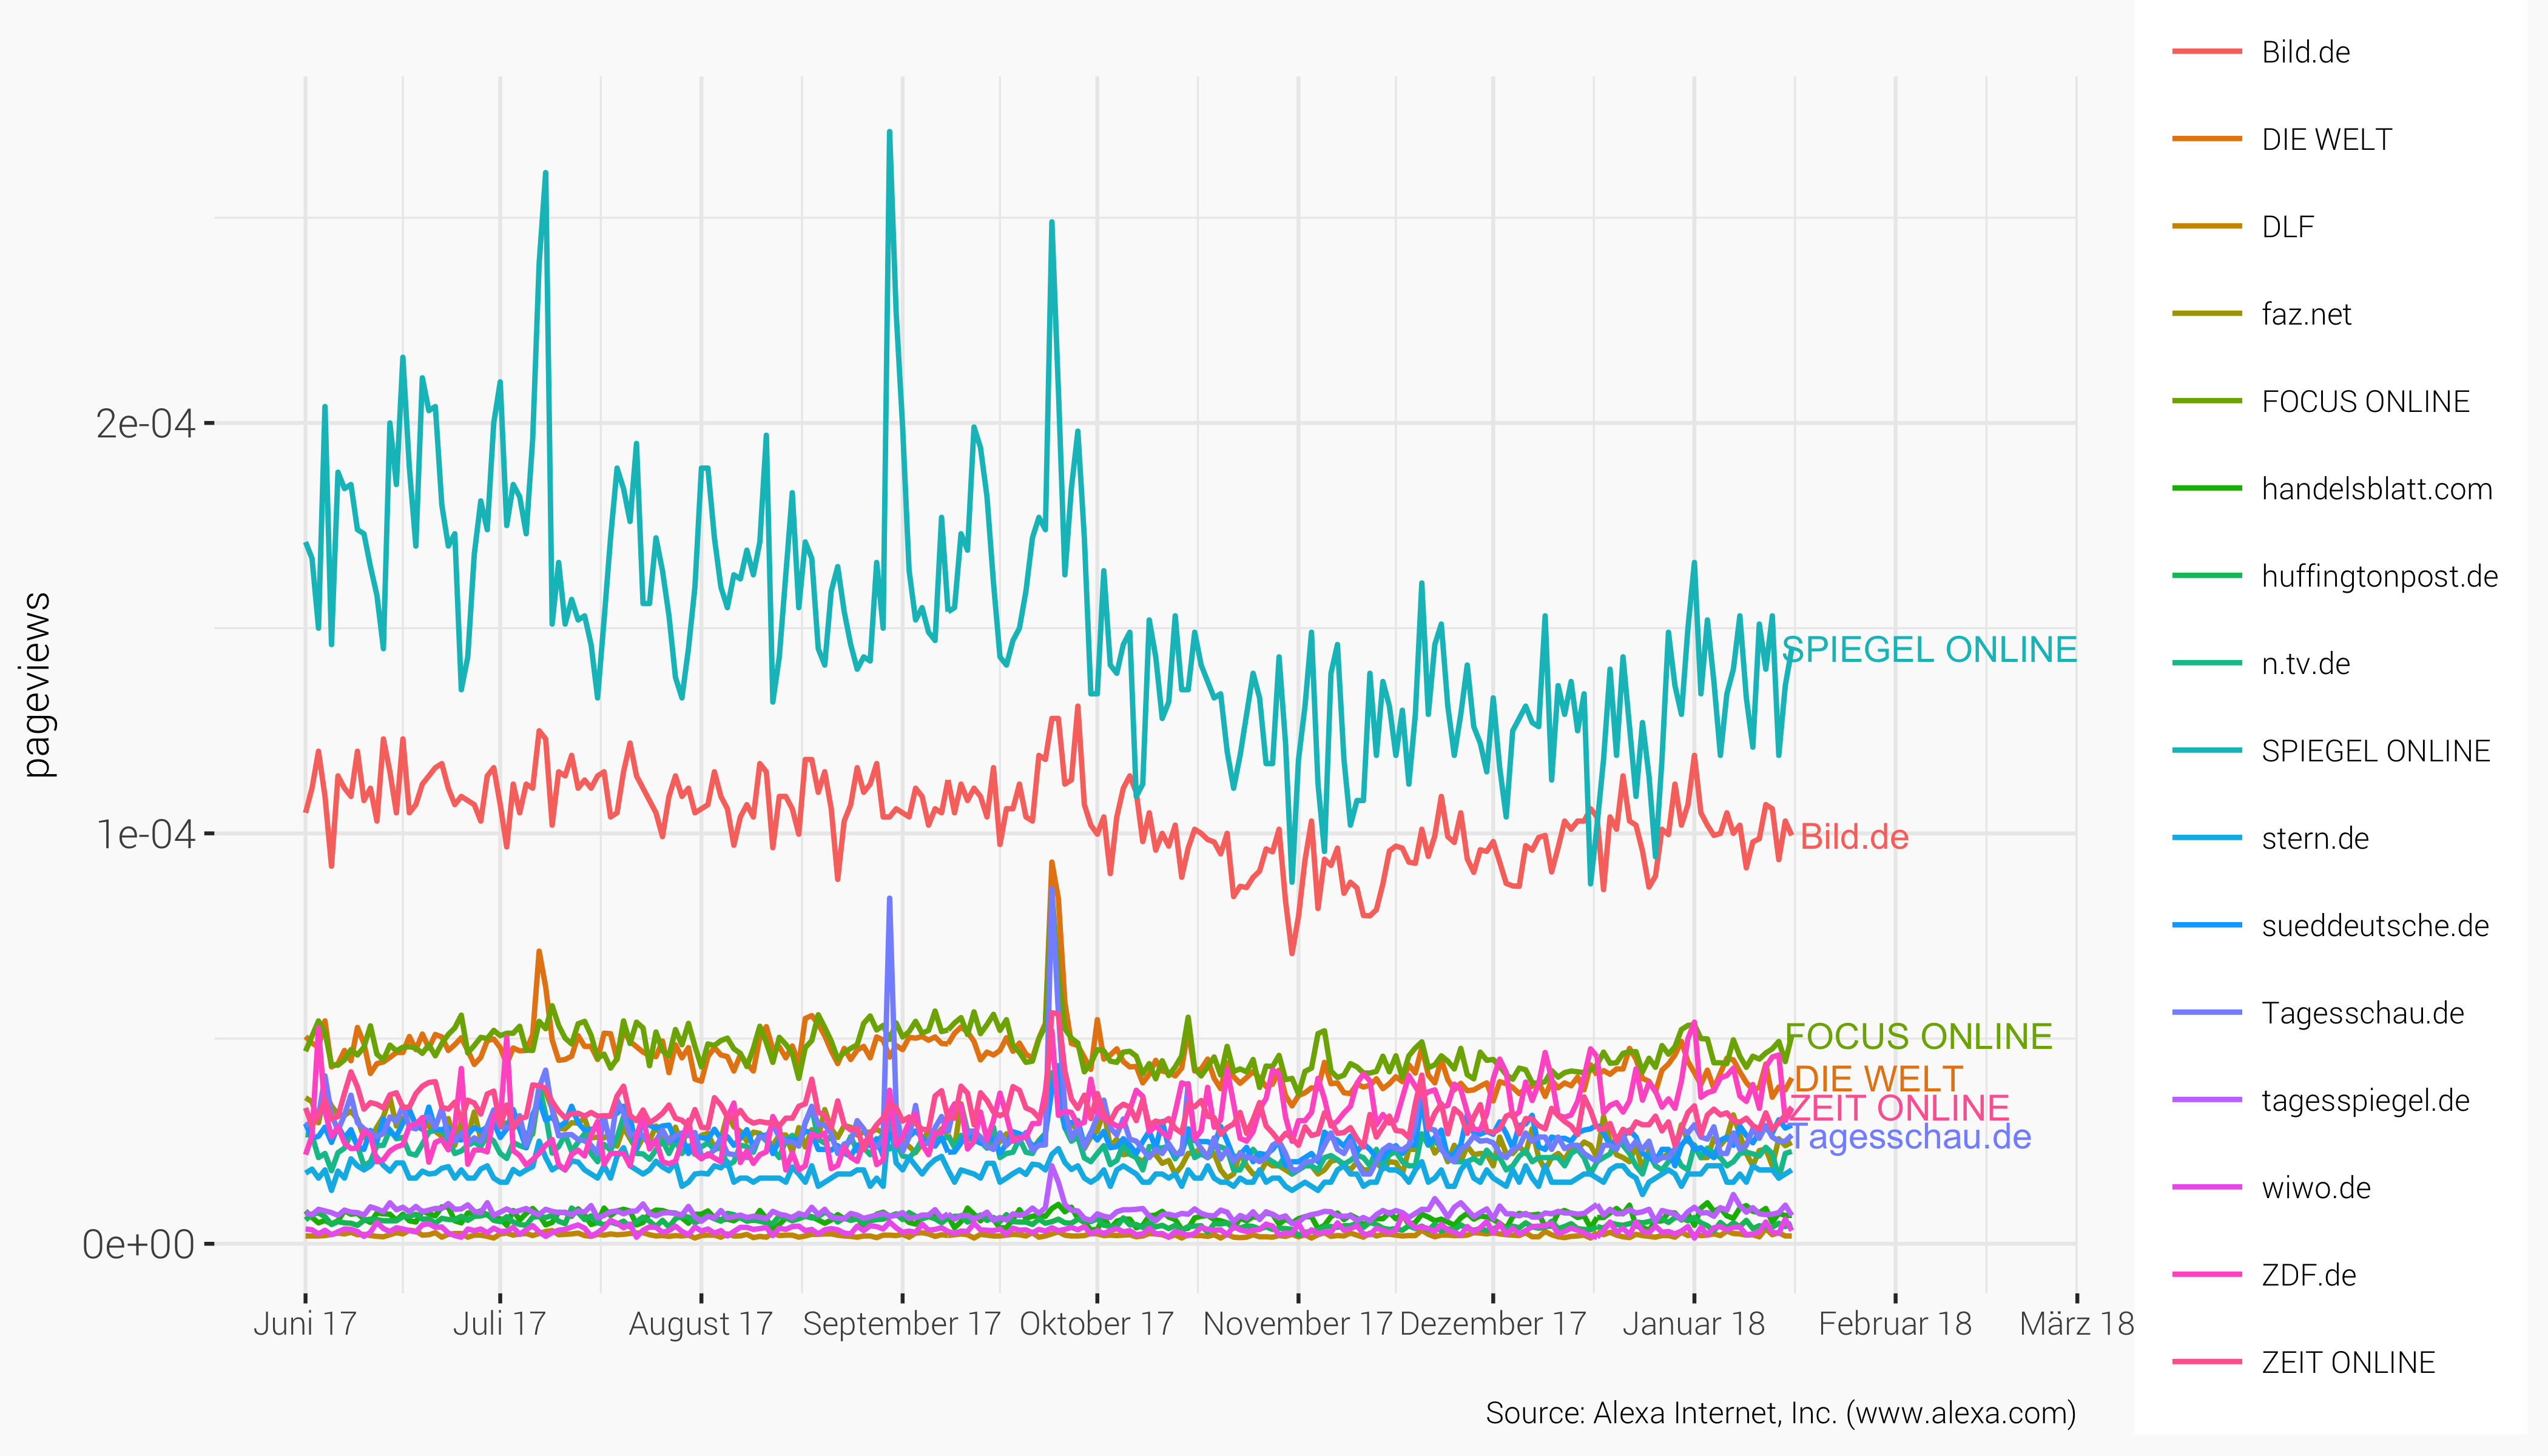
\includegraphics[width=\textwidth]{../figs/reach.png}
			\caption{Percentage of daily pageviews}
			\label{fig_reach}
		\end{subfigure}
		\begin{subfigure}[normla]{0.49\textwidth}
			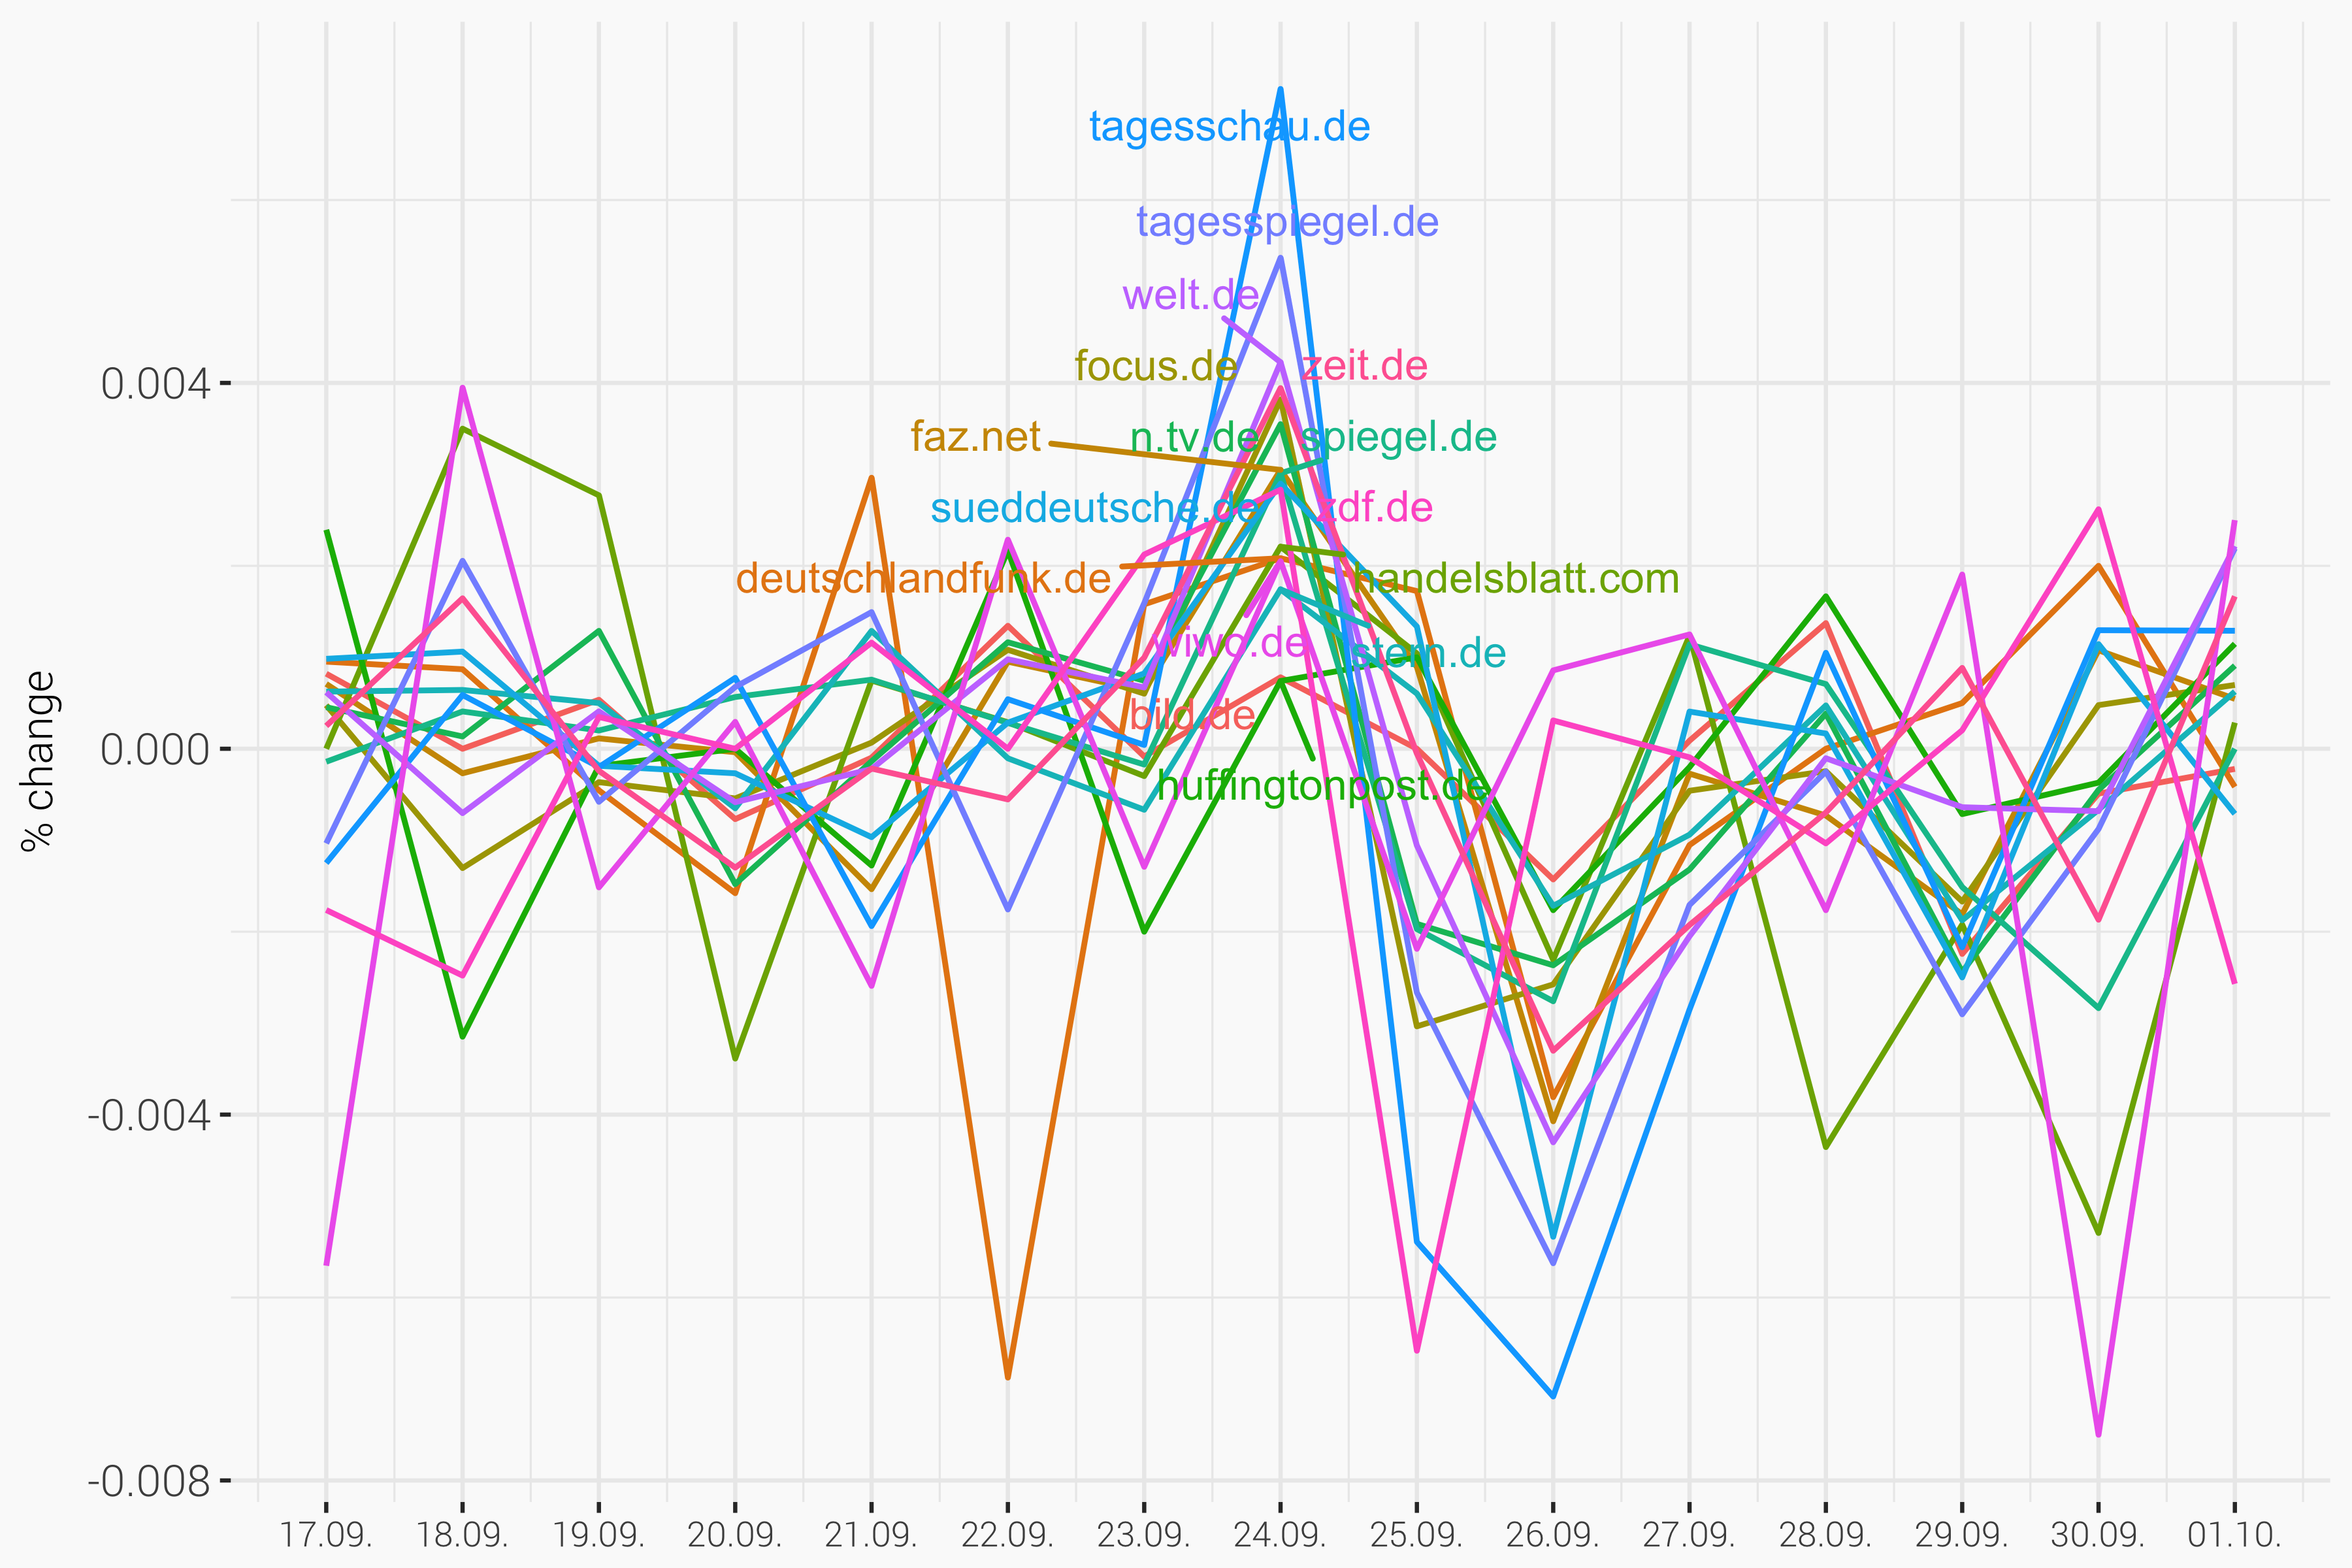
\includegraphics[width=\textwidth]{../figs/perc_change.png}
			\caption{Percentage change of pageviews}
			\label{fig_change}
		\end{subfigure}
	\end{center}
\end{figure}


Users can access a website either directly or through an intermediary, such as search engines or social media. As the figure \ref{fig_traffic} illustrates\footnote{The figure shows the percentage of total traffic by a source for the time period 18.12.2017-18.01.2017}, direct access\footnote{Direct traffic includes: Direct navigation (Someone types the website URL into a browser); Bookmarks (Clicks on a bookmark/favorite link in a browser); Email (Clicks on links in desktop email clients)} to a website is the main source of traffic for most news providers. In the case of Bild.de, the percentage is 85\%. Also n-tv.de (79\%), spiegel.de (76\%) and tagesschau.de (75\%) get most of their traffic via the direct route. Other providers are more reliant on intermediaries, mainly search engines. Focus.de, Deutschlandfunk.de, Handelsblatt.com, for example, obtain between 40\% and 45\% of its traffic via search engines. Thus, an important question is, which organic search keywords send traffic to a website. Figure \ref{fig_searchtraffic} displays the percentage of organic search referrals to a specific website that come from this keyword.\footnote{Percentage of organic search referrals in major search engines over the time span Jun-Dec 2017.} E.g., 0.78\% of all organic search referrals to handelsblatt.com come from the keyword "handelsblatt". It is not surprising that the provider's name is the keyword that generates the majority of traffic for most of the news pages. However, different topics as well as names of other providers are hidden among the top 10 keywords.   

\begin{figure}[H]
	\caption{Traffic Sources}
	\begin{center}
		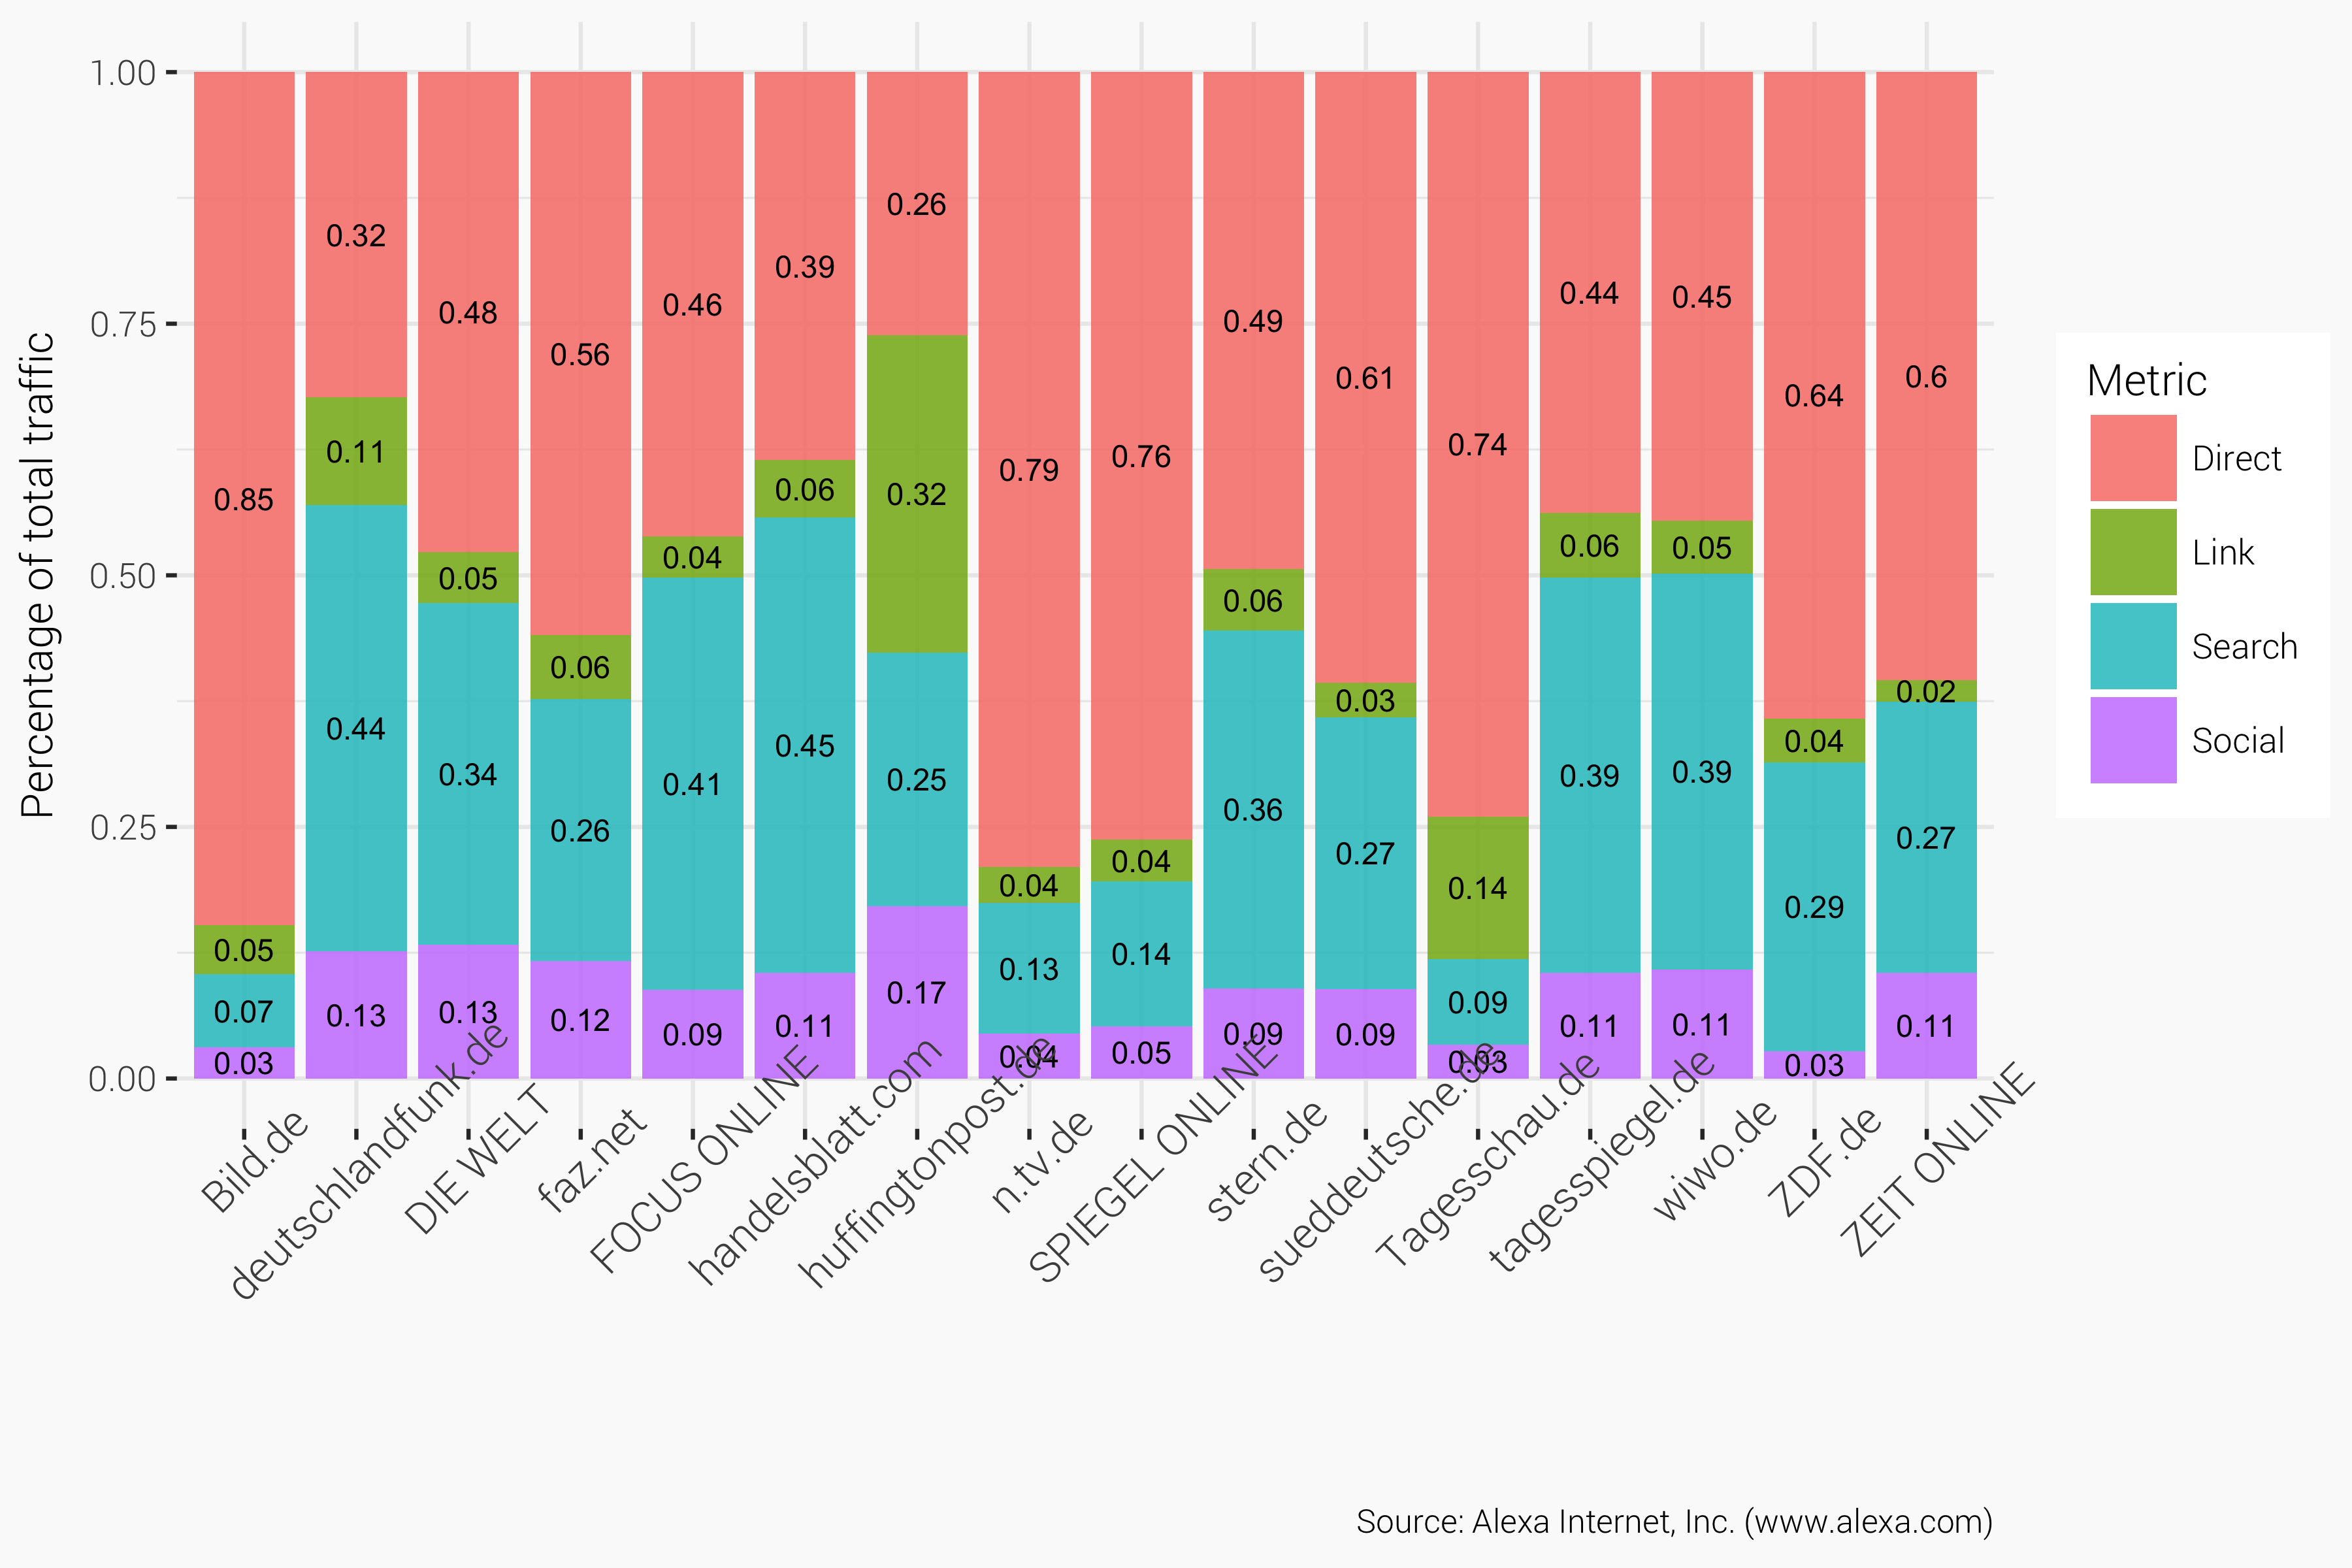
\includegraphics[width=0.8\textwidth]{../figs/traffic_source.png}
		\label{fig_traffic}
	\end{center}
\end{figure}

\begin{figure}[H]
	\caption{Search traffic \%}
	\begin{center}
		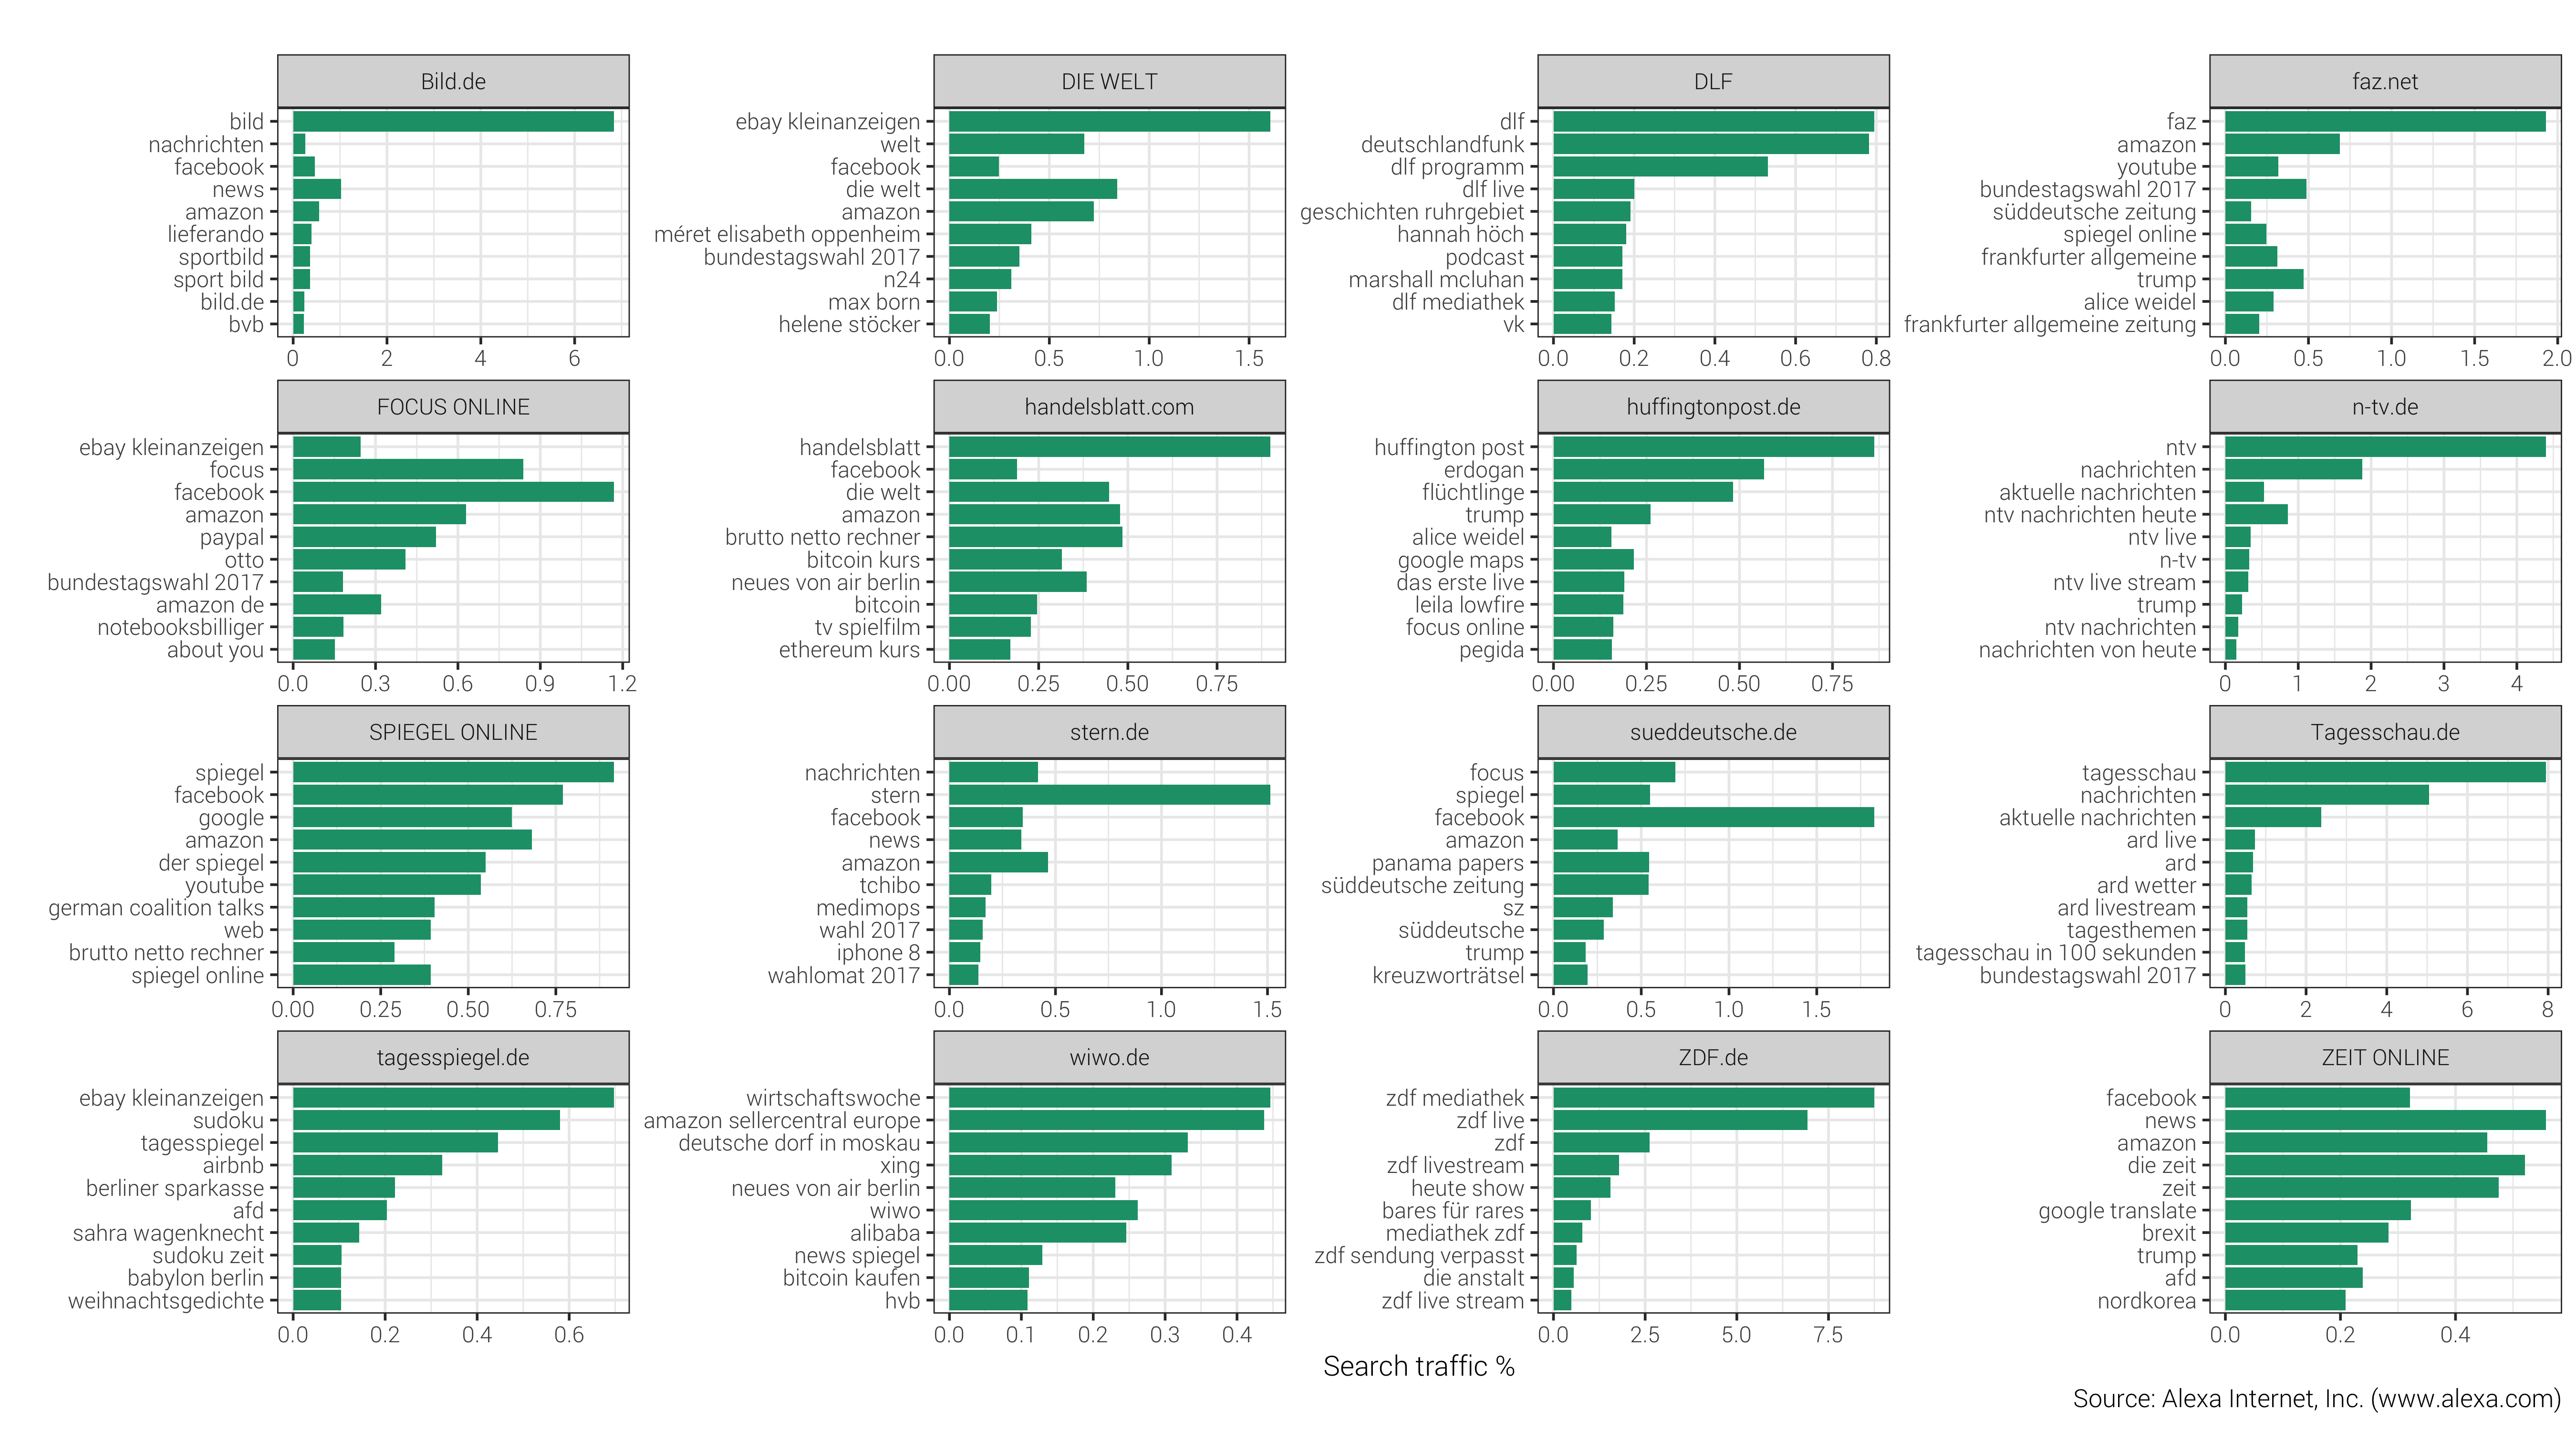
\includegraphics[width=0.95\textwidth]{../figs/search_traffic.png}
		\label{fig_searchtraffic}
	\end{center}
\end{figure}

Assuming that each search query is in itself a market where providers compete for traffic, the share of search queries for a keyword that has led visitors to a news page is the market share of that provider. In this context, figures \ref{fig_keywords1} and \ref{fig_keywords2} show the market share of providers for different keywords.\footnote{The figures show the percentage of searches for a keyword that sent traffic to a website in major search engines over the time span Jun-Dec 2017.} Nearly 15\% of all search queries for the keyword "Bundestagswahl 2017" (federal elections 2017) were forwarded to welt.de. Focus.de, faz.net and spiegel.de obtained a market share of 7\% - 8\%. For the keyword "Groko" (grand coalition between CDU/CSU and SPD), SPIEGEL ONLINE was able to gain the largest market share (17\%) in the past six months, followed by DIE WELT (\%10), FOCUS ONLINE (8\%) and Bild.de (7.5\%). Figure \ref{fig_keywords2} shows the market share of news pages for the keyword search for a specific party. Contrary to figure \ref{fig_keywords1} , the x-axes in figure \ref{fig_keywords2} are scaled equally to show not only the market share of news sites depending on one party, but also for which party this provider has the largest market share. 

\begin{figure}[H]
	\caption{Market share for different keywords}
	\begin{center}
		\begin{subfigure}[normla]{0.7\textwidth}
			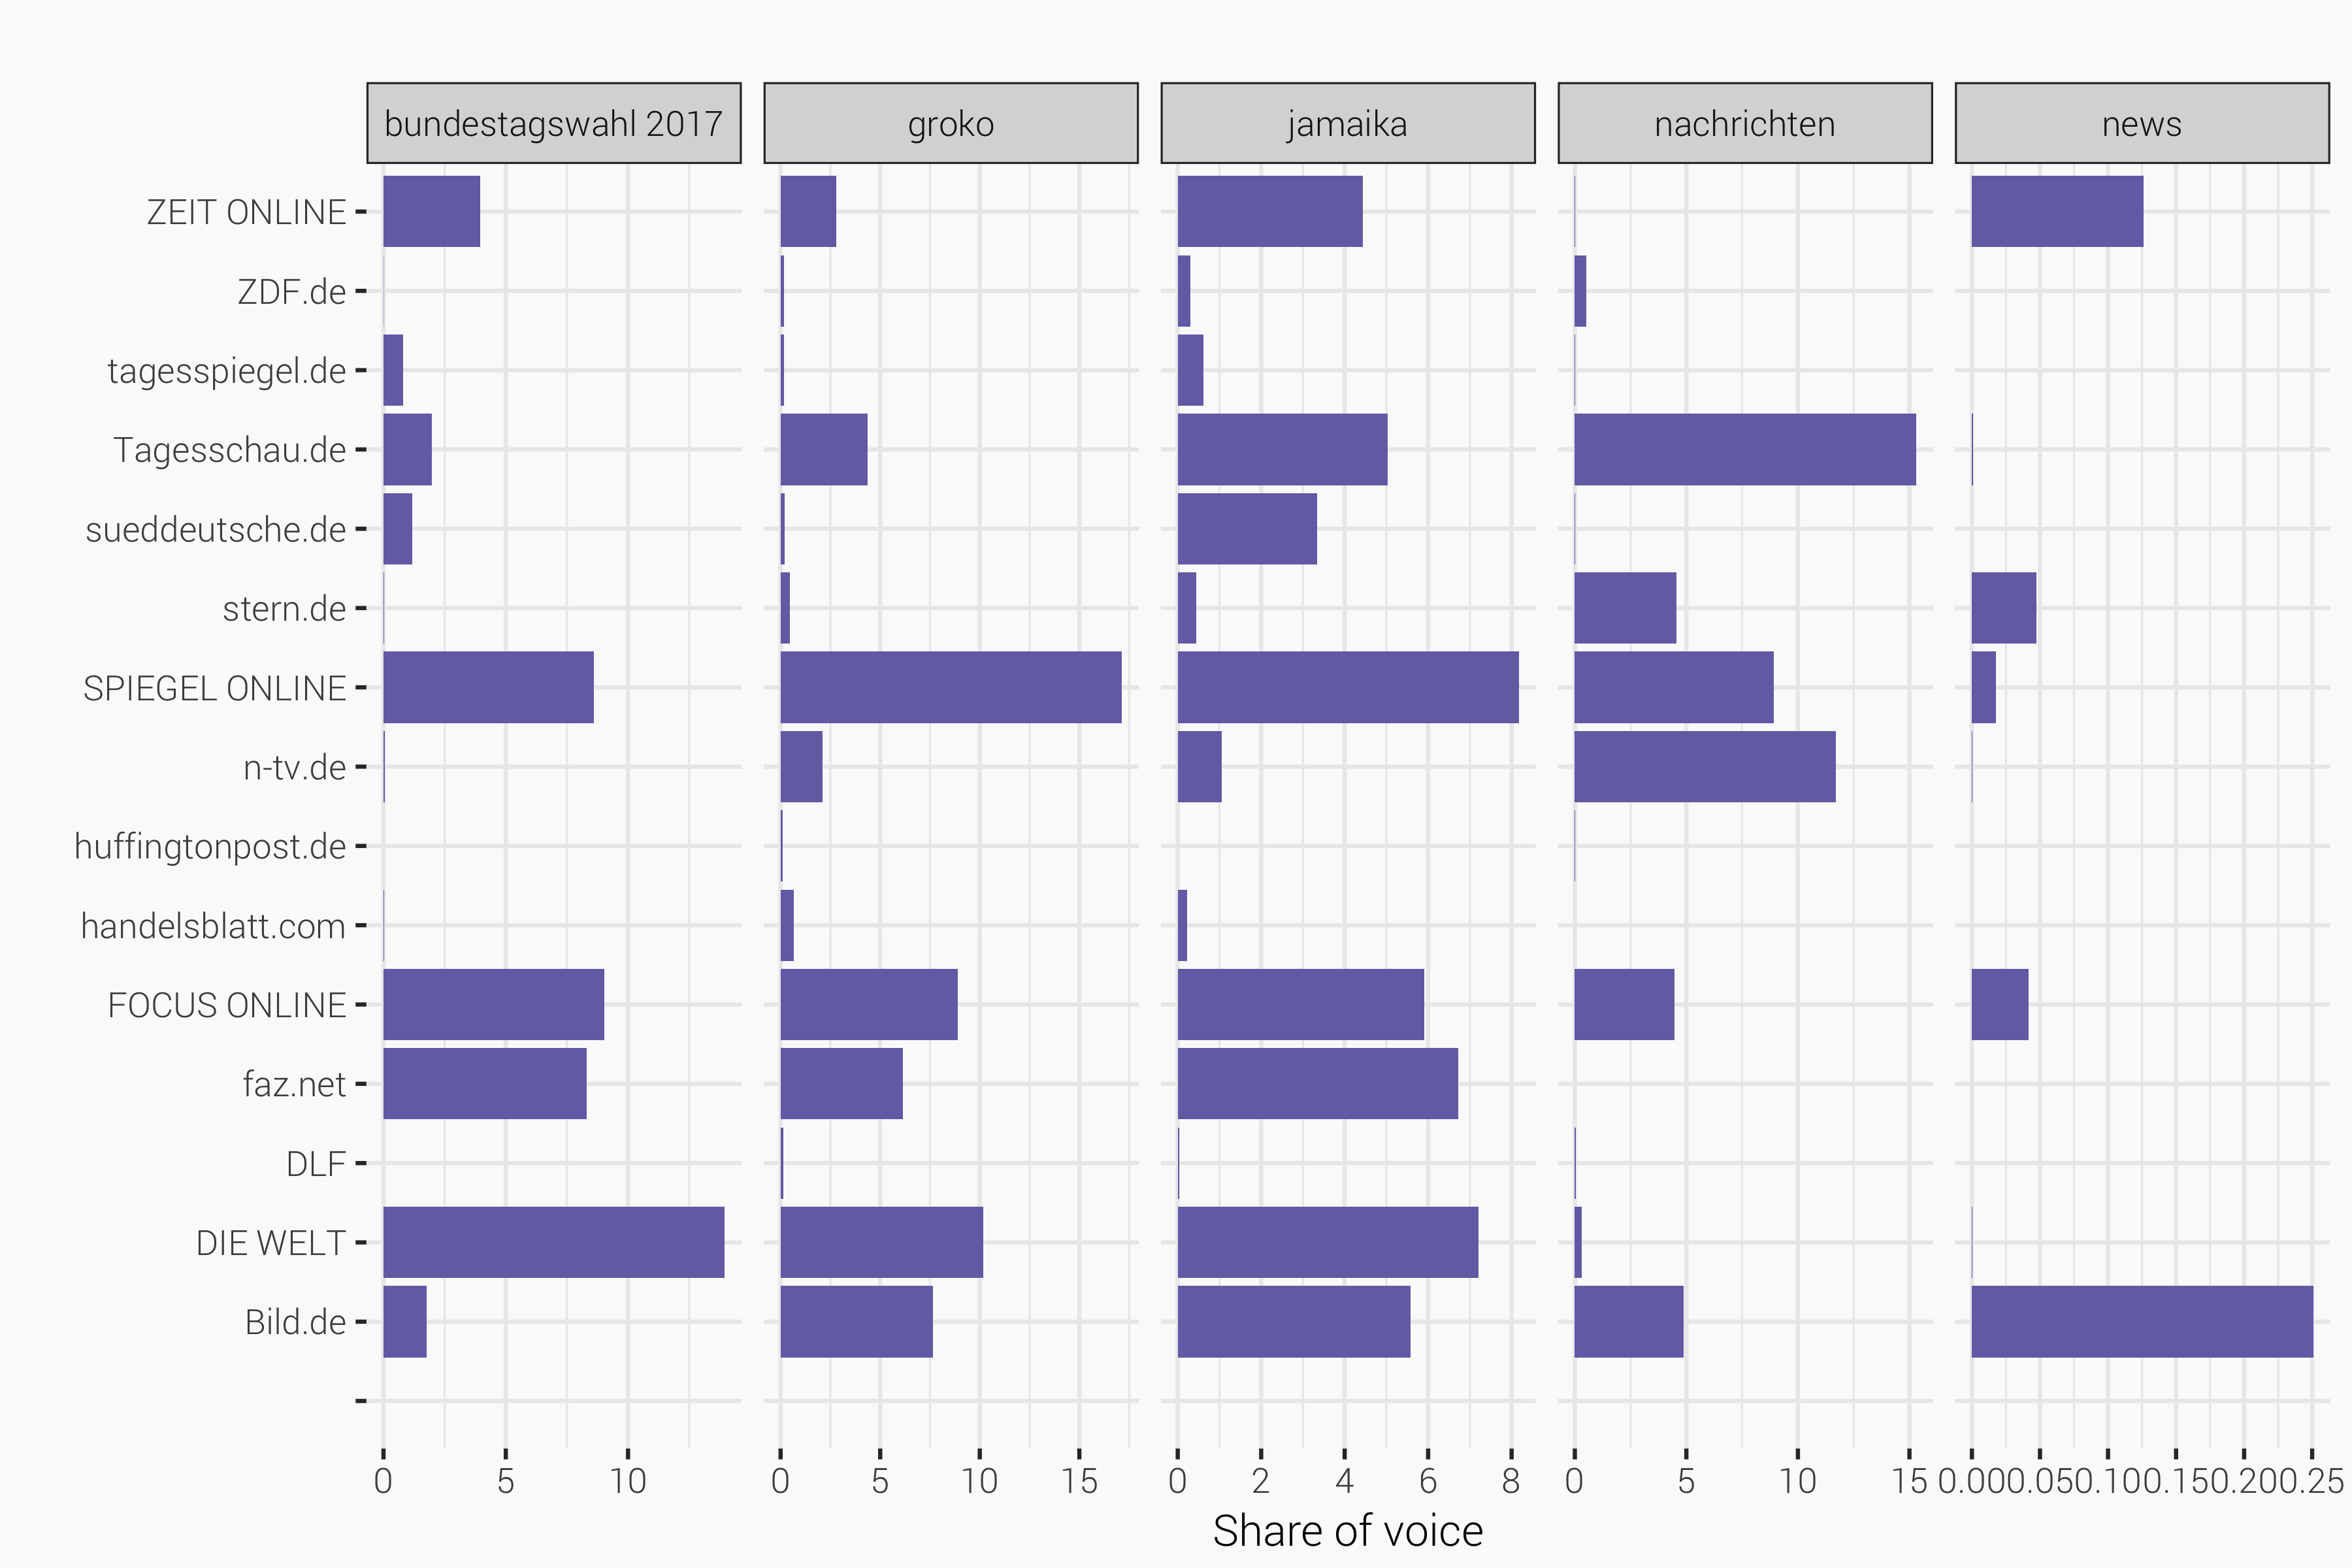
\includegraphics[width=\textwidth]{../figs/keywords1.png}
			\caption{policy topics / general}
			\label{fig_keywords1}
		\end{subfigure}
		\begin{subfigure}[normla]{0.7\textwidth}
			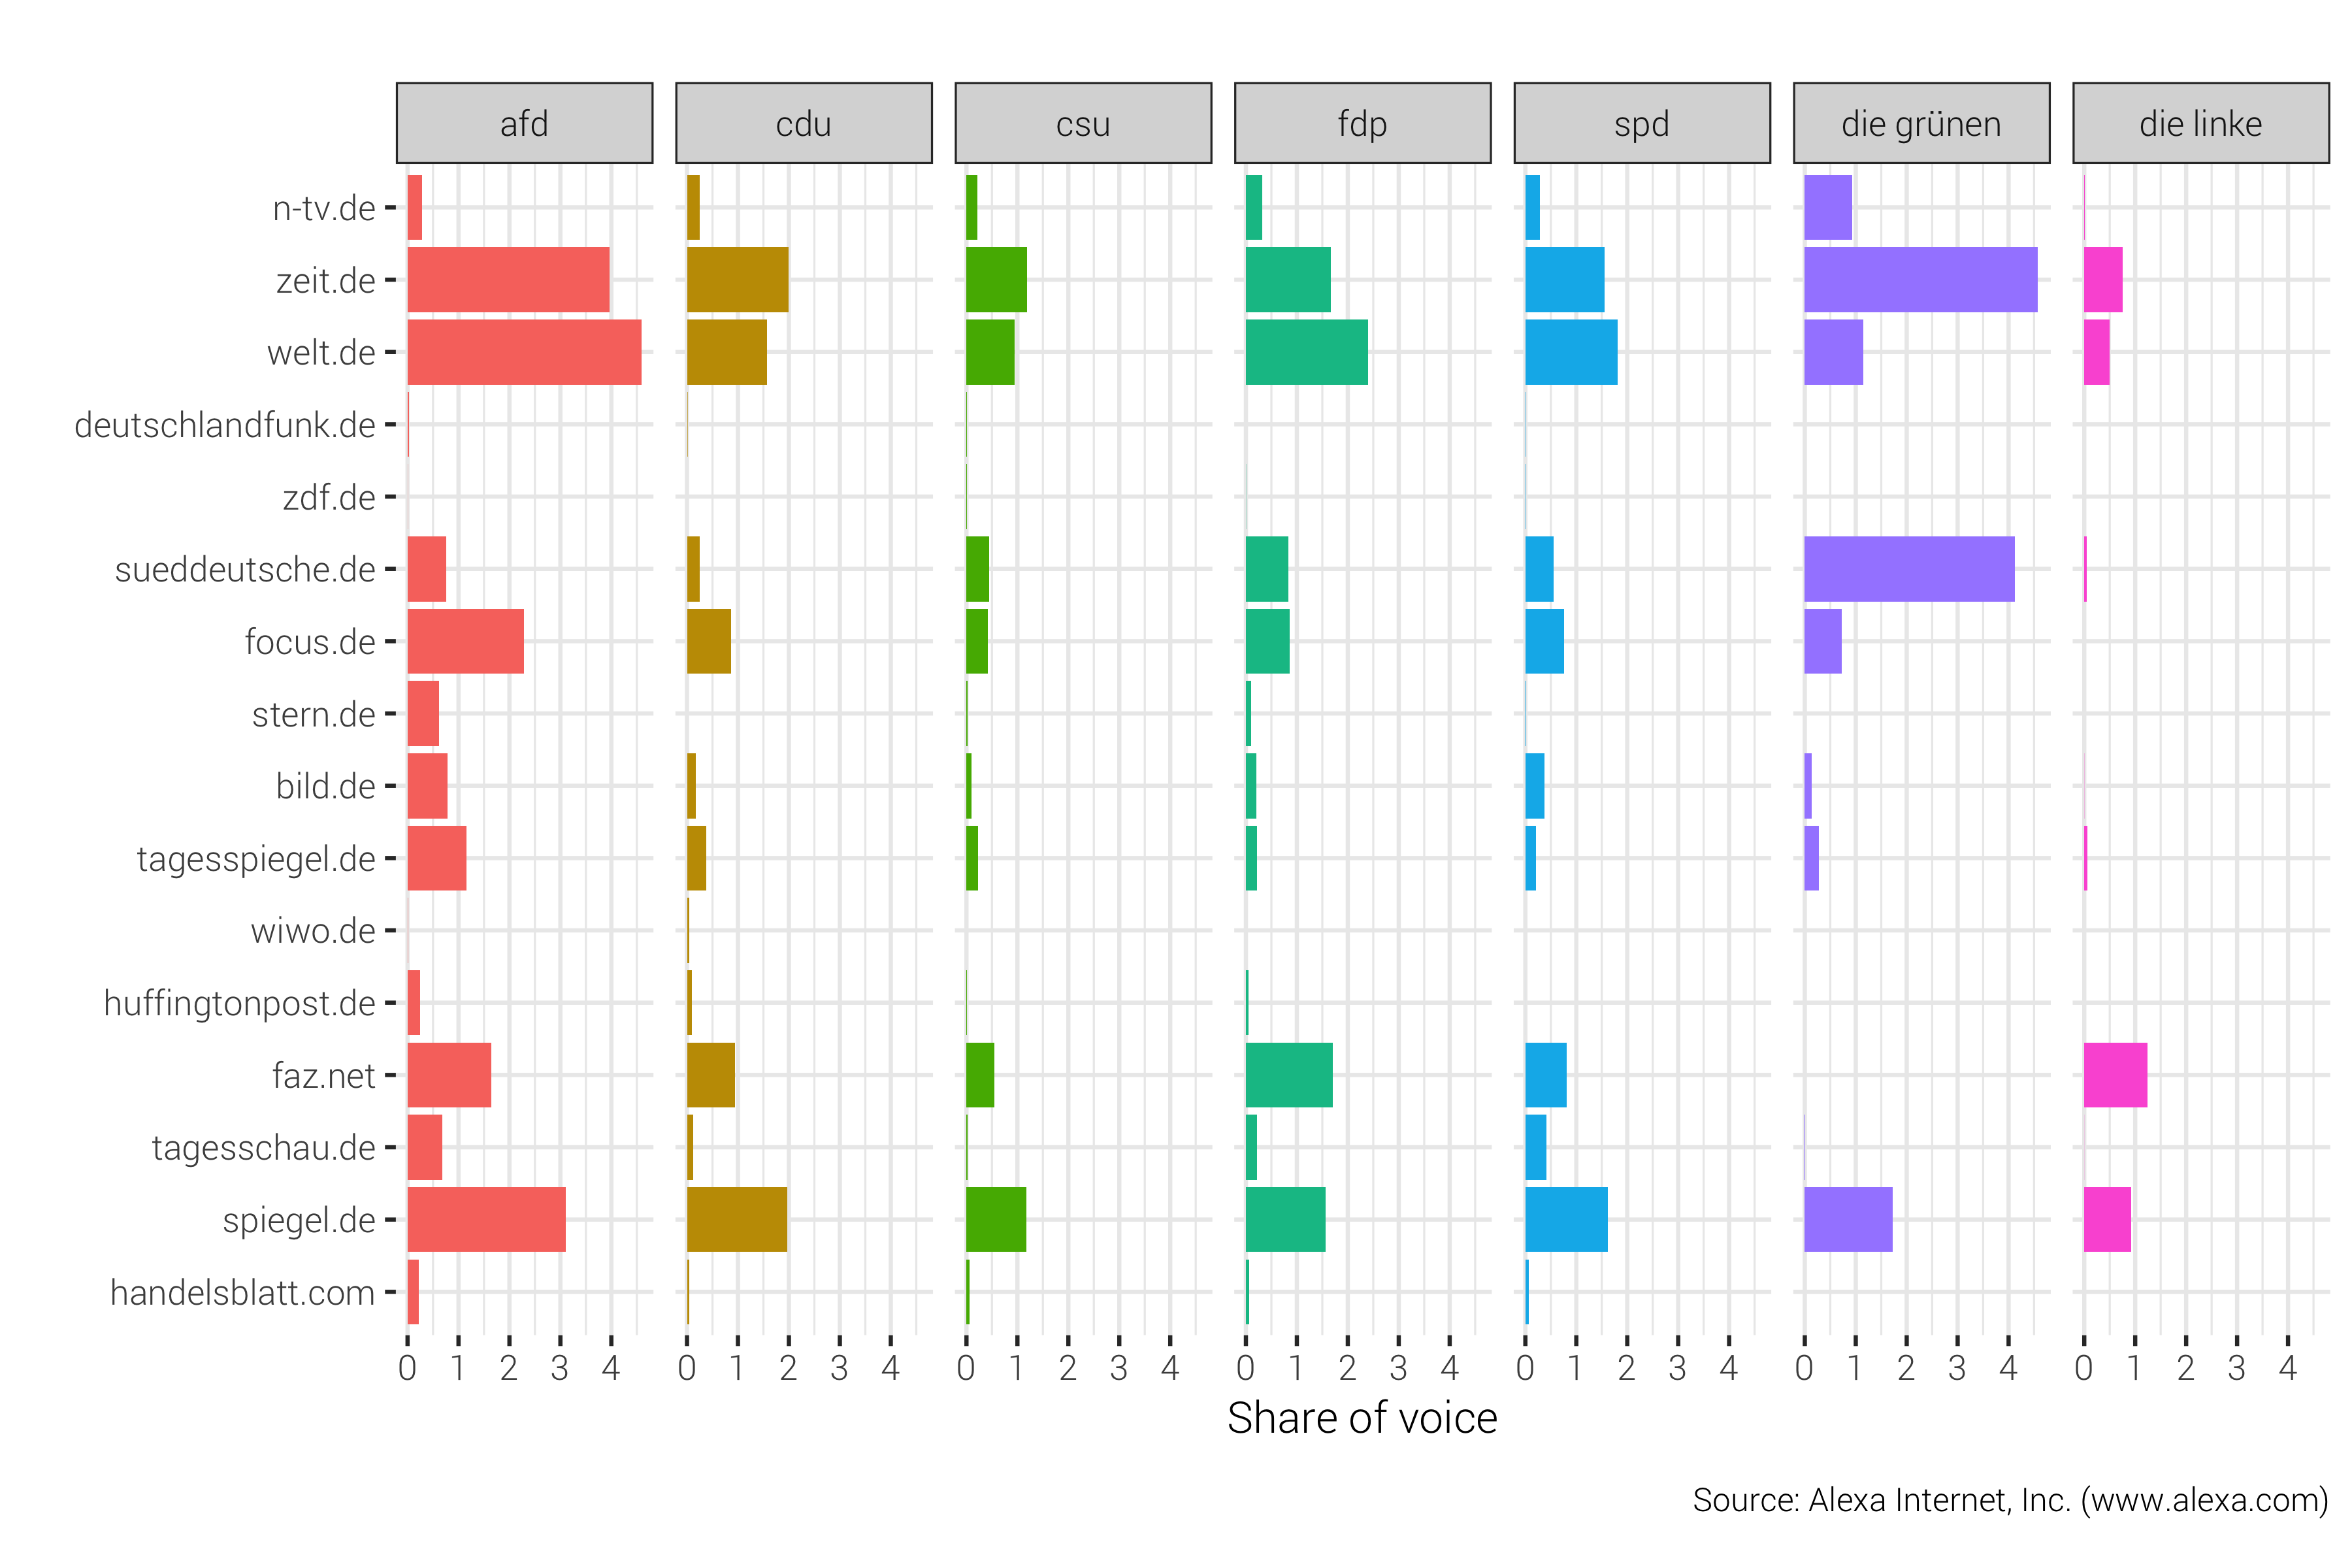
\includegraphics[width=\textwidth]{../figs/keywords2.png}
			\caption{political parties}
			\label{fig_keywords2}
		\end{subfigure}
	\end{center}
\end{figure}

% -----
% Data
% -----
\subsection{Dataset}\label{ch_data}

We conduct our estimation on a sample of 7061 online news articles from five news provider about domestic politics\footnote{Bild.de, FOCUS ONLINE, SPIEGEL ONLINE, ZEIT ONLINE, Tagesschau.de} dated from 01.06.2017 to 31.12.2017.\footnote{German federal elections took place on 24th of September 2017.} We first extract all online articles using the the Webhose.io API.\footnote{For more information see https://docs.webhose.io/v1.0/docs/getting-started. The scraping code was written in Python and can be made available on request.} We then filtered all articles from the section "domestic policy" by checking the URL structure. 

Figure \ref{fig_distr1}\footnote{The vertical line indicate the date of the federal elections (24.09.2017).} shows the distribution of the number of articles from the respective news sources by date. There is a high peak around the federal elections on September, 24th.  

\begin{figure}[H]
	\caption{Article distribution...}
	\begin{center}
		\begin{subfigure}[normla]{0.8\textwidth}
			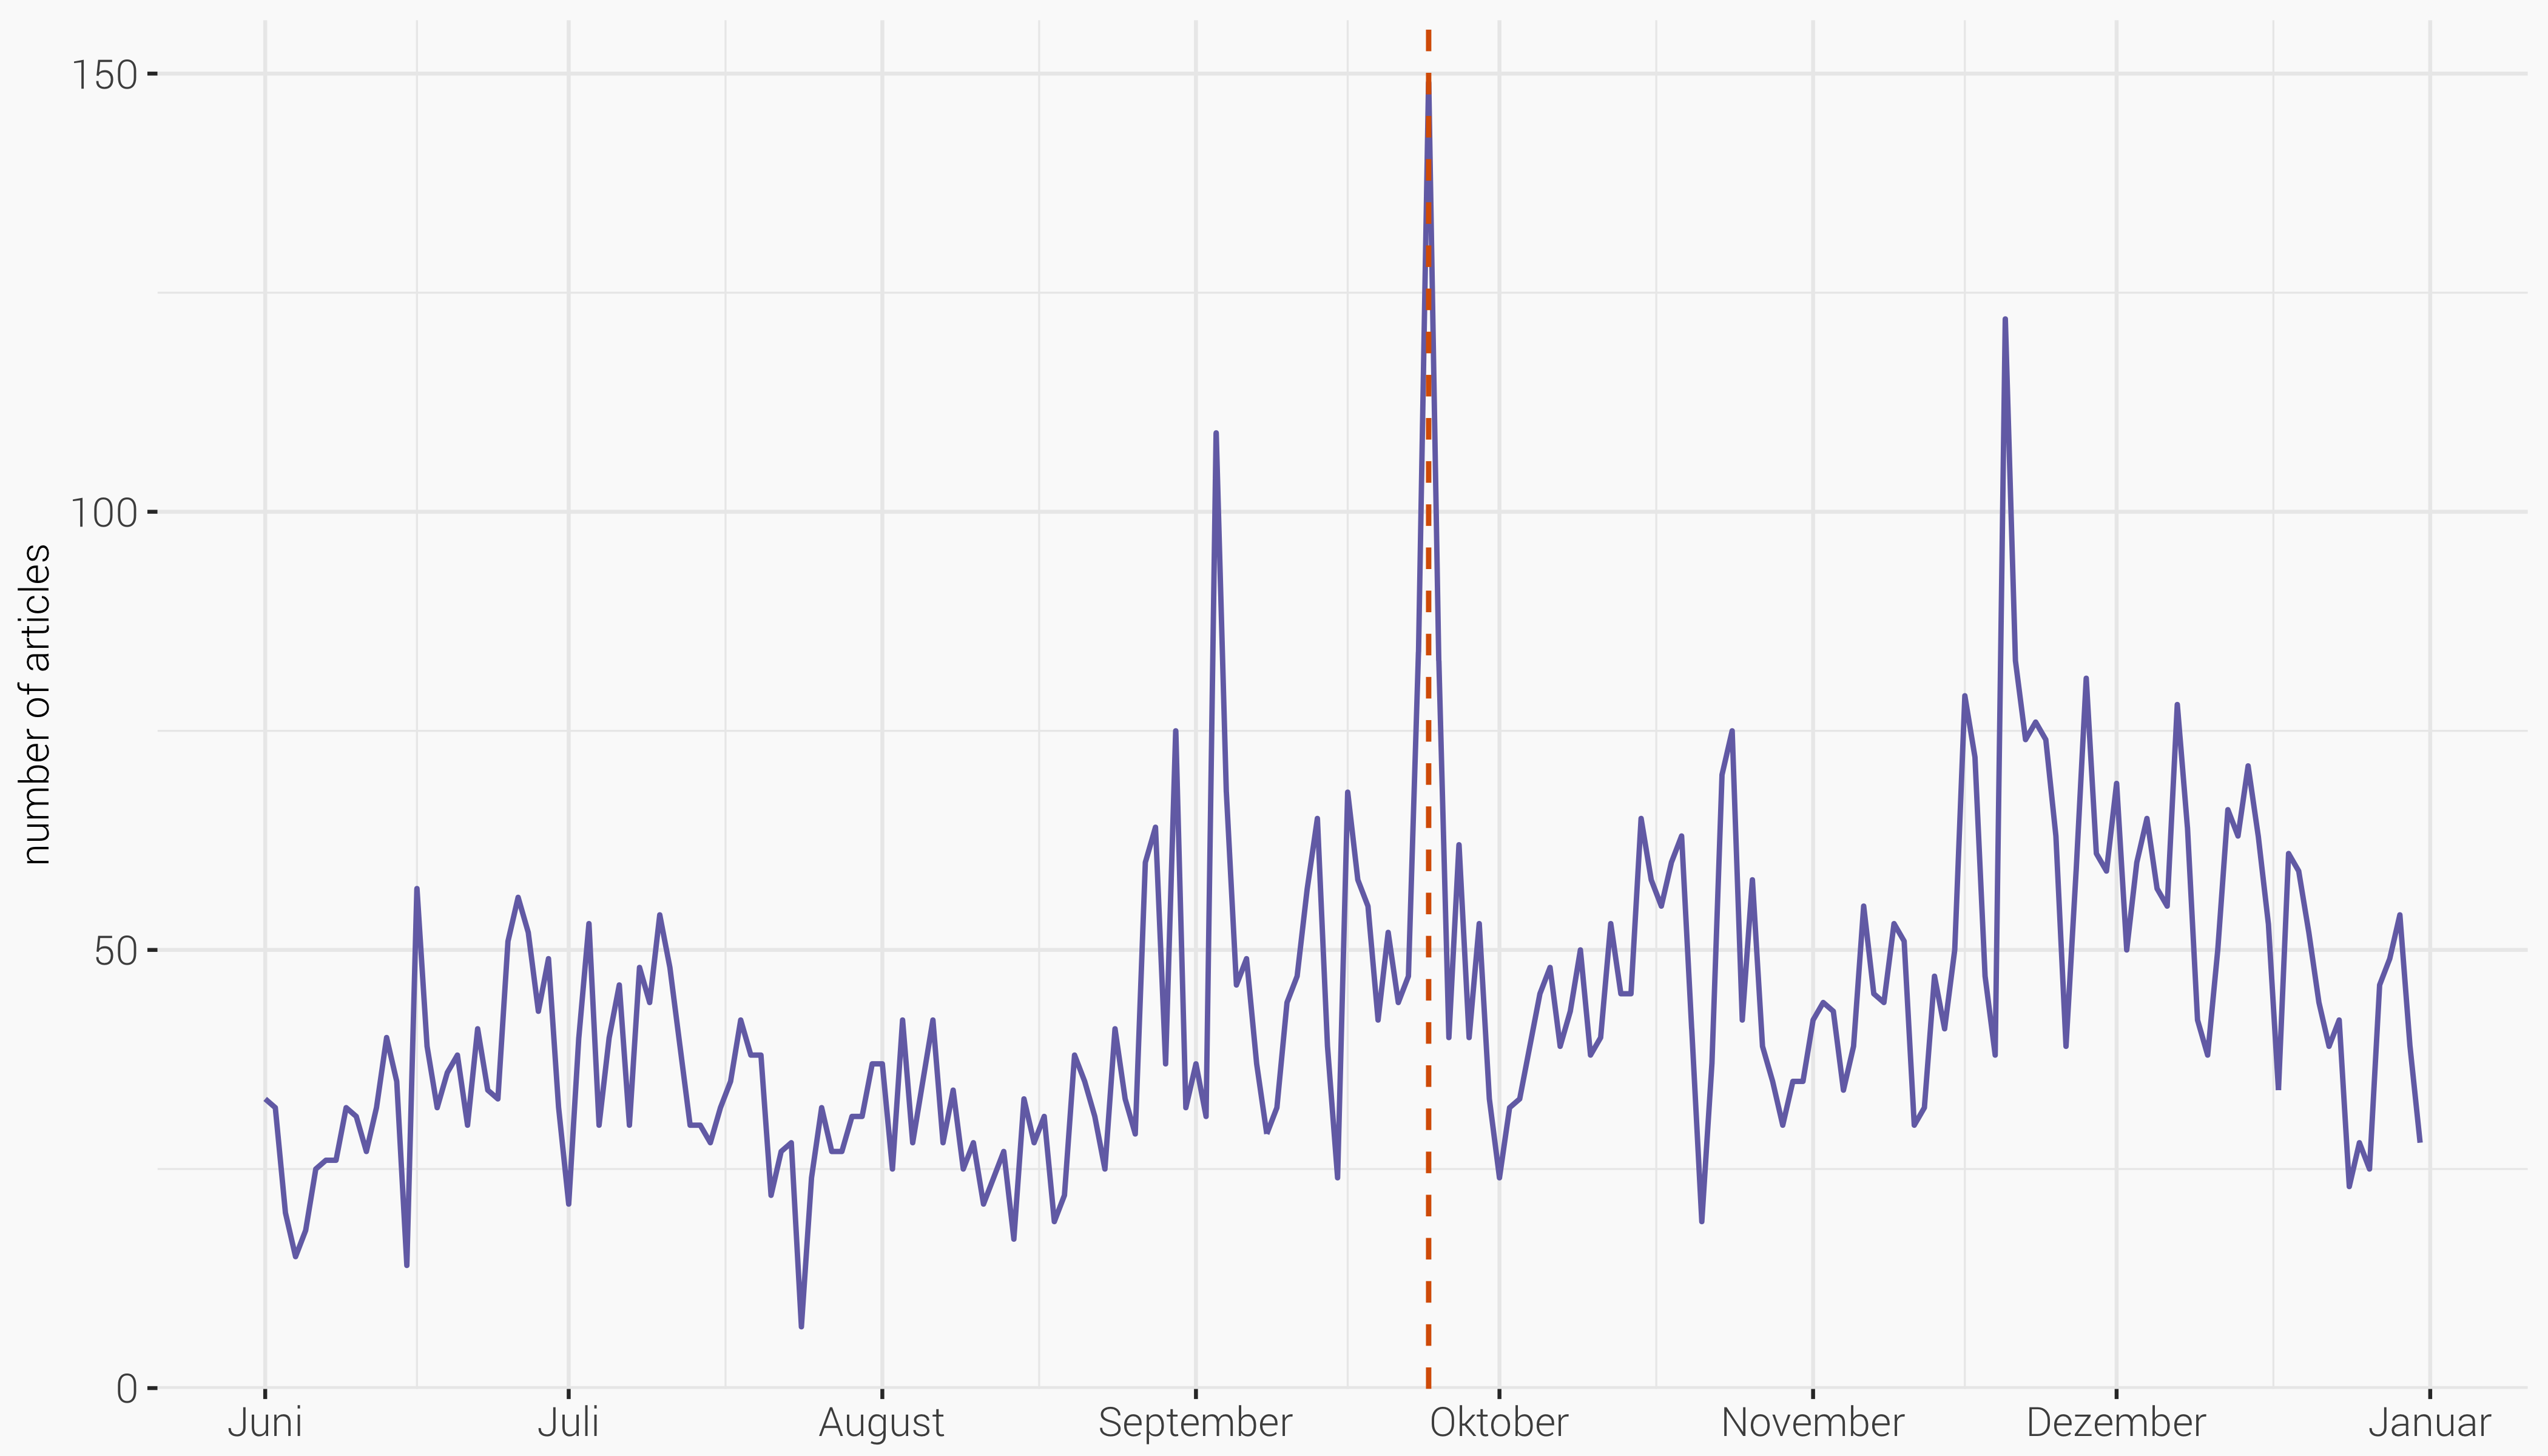
\includegraphics[width=\textwidth]{../figs/timeline.png}
			\caption{...by date \& news source}
			\label{fig_distr1}
		\end{subfigure}
		\begin{subfigure}[normla]{0.8\textwidth}
			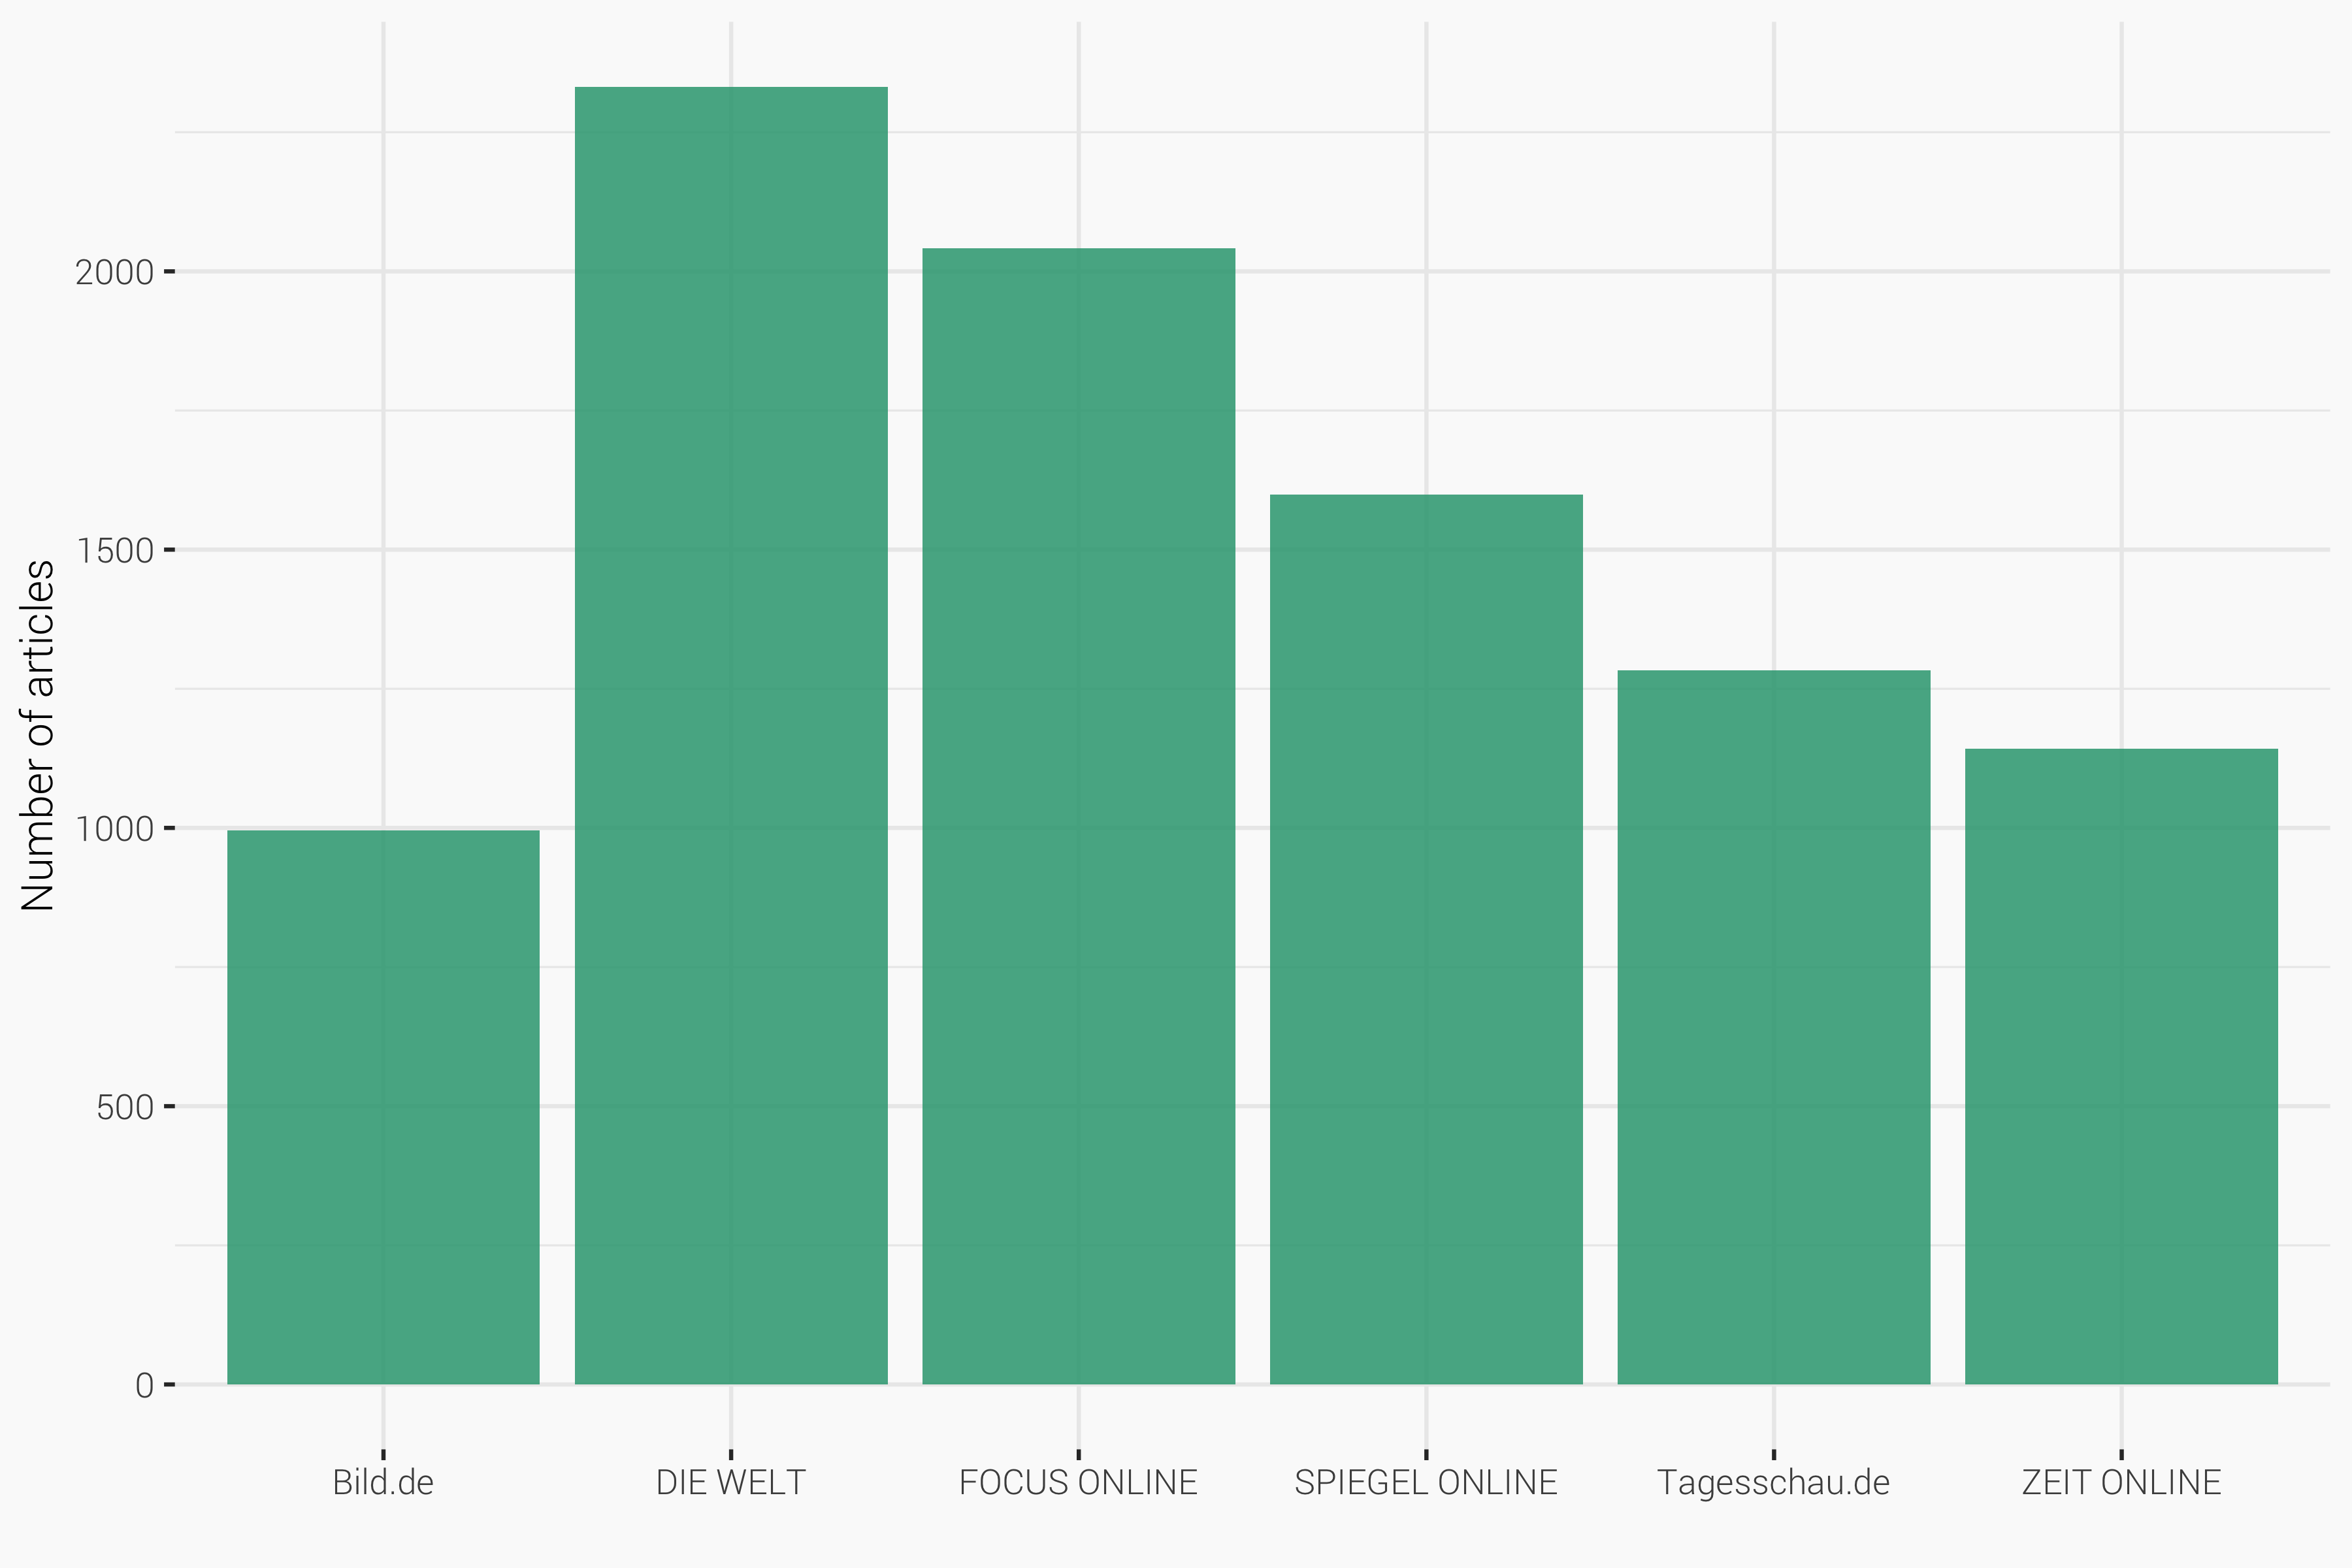
\includegraphics[width=\textwidth]{../figs/bar.png}
			\caption{... by news source}
			\label{fig_distr2}
		\end{subfigure}
	\end{center}
\end{figure}

% ------------------
% Text Pre-Procesing
% ------------------

To use text as data and reduce the dimensionality, a common strategy is to pre-process the text by imposing some preliminary restrictions (stop-word removal, tokenization) based on the nature of the data (twitter text, newspaper articles, speeches, etc.) to reduce the number of language elements to consider \citep{gentzkow_text_2017}. An overview of how these steps were applied to our data set can be found in the next section. 

After pre-processing, each document $d$ is a finite list of terms. Each unique term in the corpus is indexed by some $v \in \lbrace 1,...,V \rbrace$ where $V$ is the number of unique terms. For each document $d \in \lbrace 1,...,D \rbrace$ we compute the number of occurrences of term $v$ in document $d$ to obtain the count $x_{d,v}$. The $D$ x $V$ matrix $\boldsymbol{X}$ of all such counts is called the document-term matrix. This representation is often referred to as the bag of words model, since the order in which words are used within a document is completely disregarded. 

A central task in text mining is to extract low-dimensional information from documents that are high-dimensional by nature \citep{bholat_text_2015}. This is related to the task of reducing the number of unique language elements in order to reduce the dimensionality of data (to avoid unnecessary computational complexity and overfitting) while at the same time keeping those words that reflect the content of a document. Any useful representation of text will throw away some information, the trick is to include the relevant information for our needs, and exclude the extraneous information. 

Intuitively the term frequency (tf) of a word is a measure of how important that word may be. There are words in a document, however, that occur many times but may not be important like articles, conjunctions, and so on. These terms, often called "stop words", are important to the grammatical structure of a text, but typically don't add any additional meaning and can therefore be neglected. We use a pre-defined stop word list from the Snowball stemmer project\footnote{http://svn.tartarus.org/snowball/trunk/website/algorithms/*/stop.txt} together with a customized list of stop-words that are redundant superfluous or distorting. We also remove punctuation character (e.g. ., ,, !, ?, etc.) and all numbers from our corpus.  

% ----------------------
% Structural topic Model
% ----------------------
\section{The structural topic model}\label{ch_model}

We use the structural topic model (STM) developed by \citet{roberts_model_2016} that allows us to incorporate document specific covariates (e.g. the author or date of a document). STM is a recent extension of the standard topic modeling technique, labeled as "latent Dirichlet allocation" (LDA), which refers to the Bayesian model in \citet{blei_latent_2003} that treats each word in a topic and each topic in a document as generated from a Dirichlet - distributed prior.\footnote{See also \citet{griffiths_probabilistic_2002}, \citet{griffiths_finding_2004} and \citet{hofmann_probabilistic_1999}. \citet{pritchard_inference_2000} introduced the same model in genetics for factorizing gene expression as a function of latent populations.} Topic models formalize the idea that documents are formed by hidden variables (topics) that generate correlations among observed terms. Since its introduction into text analysis, LDA has become hugely popular and especially useful in political science.\footnote{see \citet{blei_probabilistic_2012}, \citet{grimmer_text_2013} and \citet{wiedmann_text_2016} for an overview in social science and \citet{gentzkow_text_2017} give an overview of text mining applications in economics.} \citet{wiedmann_text_2016} use topic model methods in on large amounts of news articles from two german newspapers published between 1959 and 2011, to reveal how democratic demarcation was performed in Germany over the past six decades. 

STM has been applied to multiple academic fields: \citet{roberts_structural_2014} uses STM to analyse open-ended responses from surveys and experiments, \citet{farrell_corporate_2016} applies the model to scientific texts on climate change, revealing links between corporate funding and the framing of scientific studies and \citet{mishler_using_2015} shows that "STM can be used to detect significant events such as the downing of Malaysia Air Flight 17" when applied to twitter data. Another study shows how STM can be used to explore the main international development topics of countries’ annual statements in the UN General Debate and examine the country-specific drivers of international development rhetoric \citep{baturo_what_2017}. \citet{mueller_reading_2016} uses newspaper text to predict armed conflicts in different regions. They use the estimated topic shares in linear fixed effects regression to forecast conflict out-of-sample.

% Topic Modeling
% --------------
\subsection{Generative Process of STM}

The following description of the generative model of the STM is based on \citet{roberts_structural_2013} and \citet{roberts_stm:_2016}. The process of filling a word-position in a document begins with the generation of a document-specific topic-prevalence vector $d(\boldsymbol{\theta}_d)$ drawn from a logistic-normal distribution, where the parameters are a function of the covariate values:

\begin{align*}
	\boldsymbol{\theta}_d|\boldsymbol{x}_{d\gamma},\boldsymbol{\Sigma} \sim \textrm{LogisticNormal}(\mu = \boldsymbol{x}_{d\gamma}\boldsymbol{\Sigma})
\end{align*}

$\boldsymbol{x}_d\gamma$ lists the values of all metadata covariates for document $d$, where $\gamma$ relates these covariate values to the topic-prevalence. The structure of $\boldsymbol{\Sigma}$ implies the possibility of correlations across documents in the topic-prevalence vector which help enhance interpretation and prevent overfitting. 

Given the document-specific distribution over topics, for each word in the document ($n \in \lbrace 1,...,N_d\rbrace$) is assigned to a specific topic $z_{dn}$ through the process

\begin{align*}
	z_{dn}|\boldsymbol{\theta}_d \sim \textrm{Multinomial}(\boldsymbol{\theta}_d)
\end{align*}

where the $k^{th}$ element if $z_{dn}$ is unity and all other elements are zero when topic $k$ is chosen. 

Conditional in the topic chosen, a specific word, $w_{dn}$, is chosen from the overall corpus vocabulary $V$ to fill position $n$ in document $d$, using the following process:

\begin{align*}
	w_{dn}|z_{dn},\beta_{dkv} \sim \textrm{Multinomial}(\beta_{dk1},...,\beta_{dkV}).
\end{align*}

where the word probability $\beta_{dkv}$ is modeled as a function of the two parameters $m_v$ (indicating the importance of that word across all documents) and $\kappa_{kv}$ (indicating the importance of the word given the topic $k$). Transforming the sum of these coefficients into probabilities for use in a multinomial distribution via logistic transformation, one obtains:

\begin{align*}
	\beta_{dkv}|z_{dn}\propto\textrm{exp}(\boldsymbol{m}_v+\kappa_{kv})
\end{align*}


% ----------------------
% Model Selection
% ----------------------
\subsection{Model and parameter selection}

Topic models are usually imprecise as a number of assumptions have to be made that influence the performance of the classification task. Furthermore, multiple solutions exist for the optimization problem. The STM maximizes the posterior likelihood that the observed data were generated by the above data-generating process using an iterative approximation-based variational expectation-maximization algorithm\footnote{A technical description of this maximization process can be found in \citet{roberts_model_2016}} available in R's stm package \citep{roberts_stm:_2016}. Regularizing prior distributions are used for $\gamma$, $\kappa$ and $\Sigma$. Since an ex ante valuation of a model is hardly possible, we compute a variety of different models with different parameters and compare them with respect to the research problem \citep{gentzkow_text_2017}. To evaluate the accuracy of a model its perplexity can be computed. Similar to cross-validation (VC), different model specifications are compared to how well they do in predicting words within a document \citep{asuncion_smoothing_2012}, \citep{wallach_evaluation_2009}. However, \citet{chang_reading_2009} have proven with large user studies that optimal held out likelihood does not correspond to human perception of semantic coherence of topics. \cite{mimno_optimizing_2011} introduced a measure of coherence of a topic by observing co-occurences of the top $N$ terms of each topic on a document. Another strategy for selecting an appropriate model is to check for residual overdispersion of the variance of the multinomial within the data generating process of the model \citep{taddy_estimation_2012}. Other approaches can be found in \citet{airoldi_reconceptualizing_2010} and \citet{teh_hierarchical_2006}. However, cross-checking some subset of assigned topic distributions to evaluate whether the estimates align with the concept of interest \citep{gentzkow_text_2017}. We apply these manual audits together with numeric optimization based on the topic coherence measure suggested by \citet{mimno_optimizing_2011}. 

This process revealed that a model with 25 topics best reflects the structure in the corpus. Furthermore, we use the source of each article (the media house) and the month it was published as covariates in the topic prevalence portion of the model. In other words, the probability distribution of topics depends on the editorial strategy of a media house as well as on the month the article was published. To address problems due to non-convexity, we rely on the spectral initialization approach advocated by \citet{roberts_navigating_2016}. 

% ----------------------
% Model Results
% ----------------------
\subsection{Empirical Evaluation}

Inference of mixed-membership models, such as the one applied in this paper, has been a thread of research in applied statistics in the past few years \citep{blei_latent_2003} \citep{erosheva_mixed-membership_2004} \citep{braun_variational_2010}. As the posterior can be highly dependent on the model definition, using multiple starting points and clever initialization are successful practices. The takeaway from empirical evaluations of the inference task of mixed-membership models is that the bayesian posterior as good frequentist properties \citep{wallach_evaluation_2009}. \citet{roberts_model_2016} use empirical evaluation, including a frequentist coverage analysis and compare the performance of their STM to a variety of alternatives in \citet{roberts_navigating_2016}. 

Figure \ref{fig_topic_proportion} displays the topics ordered by their expected frequency across the corpus. To assign a label to each topic, we used a combination of most frequent words in that topic and words with the highest "score", computed as the log frequency of the word in the topic divided by the log frequency of the word in other topics \citep{roberts_stm:_2016}. The most common topic (3) is a general topic full of words that are frequently used in policy news, and therefore is not very interpretable. However, the remaining labels seem to classify a certain topic.  

\begin{figure}[H]
	\begin{center}
	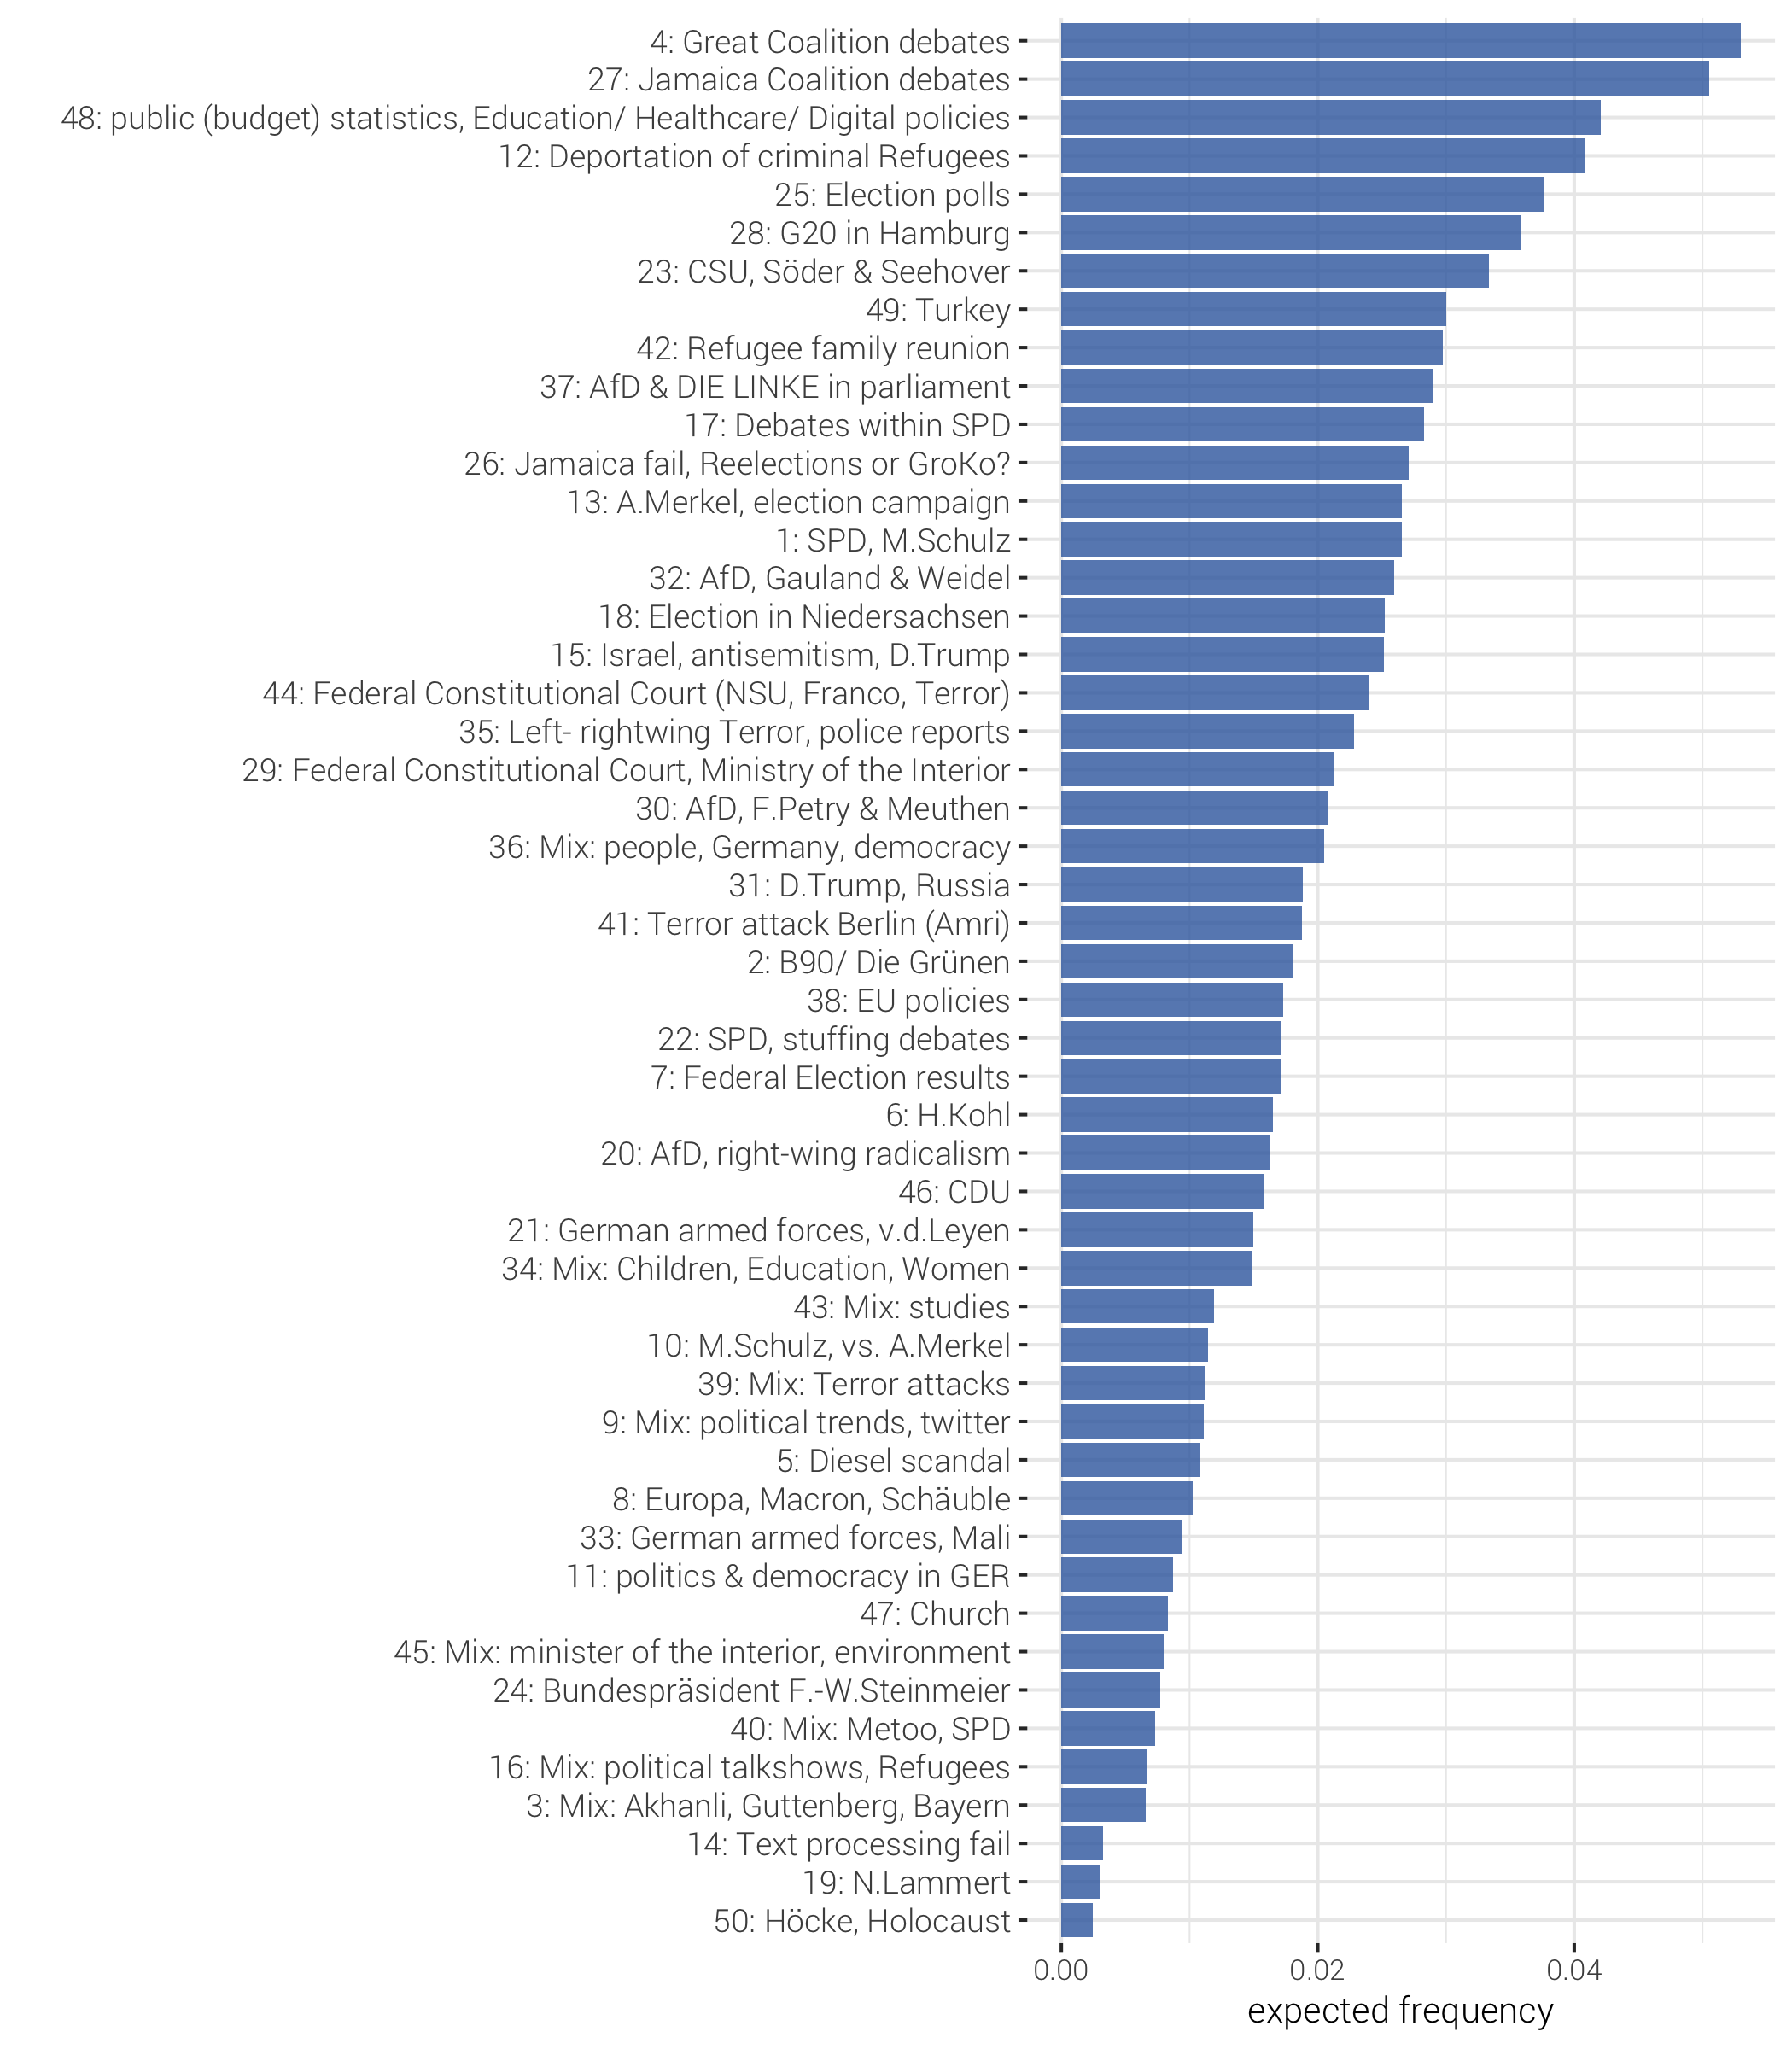
\includegraphics[width=0.8\textwidth,keepaspectratio]{../figs/topic_proportion.png}
	\caption{Expected Topic Proportion}
	\label{fig_topic_proportion}
	\end{center}
\end{figure}

% ----------------------
% Effect of covariates
% ----------------------
Since we included news source as a covariate in estimating topical prevalence part within the model, we can estimate the frequency a topic is discussed within a news corpus \citep{roberts_model_2016}. We estimate the conditional expectation of topic prevalence for given document characteristics. More specifically, we estimate a linear model, where the documents are observations, the dependent variable is the posterior probability of a topic and the covariates are the metadata of documents. The stm-package provides a function that uses the method of composition to incorporates uncertainty in the dependent variable, drawing a set of topic proportions from the variational posterior repeated times and compute the coefficients as the average over all results. 

Figure \ref{fig_estimateEffects_small} displays topics, where the most significant differences between the news sources are discernible.\footnote{An overview of all estimated topics can be found in the appendix \ref{fig_estimateEffects_full1} and \ref{fig_estimateEffects_full2}.} Topic 2, classifying articles about the diesel scandal, the glpyphosate decision and green policies, occur comparatively more often in tagesschau.de and bild.de, whereas tagesschau.de reports comparatively little about the riots during the G20 summit (topic 9). Topics 10 (about public (financial) statistics) and 13 (about the federal migration office (BAMF), asylum procedures and other issues related to refugees) also seems to be represented comparatively frequently in the tagesschau.de corpus, the latter topic is most often discussed in the DIE WELT corpus. However, topic 20 (the public debate between Die Grünen and FDP in the process of coalition negotiations) is represented significantly more often in the corpus of spiegel.de and bild.de. Topic 26, which classifies articles that deal with terrorism, mainly about the NSU trial and the main defendant Zschäpe as well es IS, is significantly more often present in the corpus of FOCUS ONLINE.

\begin{figure}[H]
	\caption{Mean prevalence of topics within each news source corpus}
	\begin{center}
		\begin{subfigure}[normla]{0.3\textwidth}
			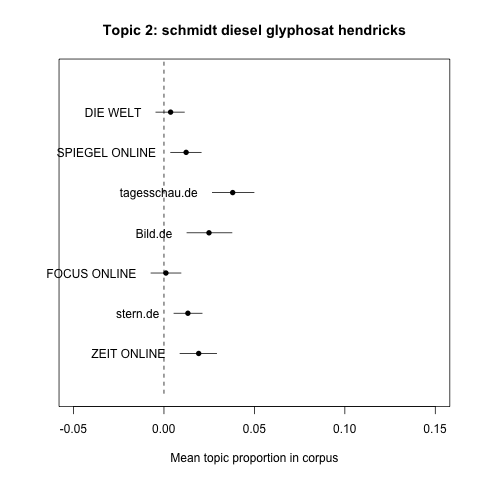
\includegraphics[width=\textwidth]{../figs/estimate_effect2.png}
		\end{subfigure}
		\begin{subfigure}[normla]{0.3\textwidth}
			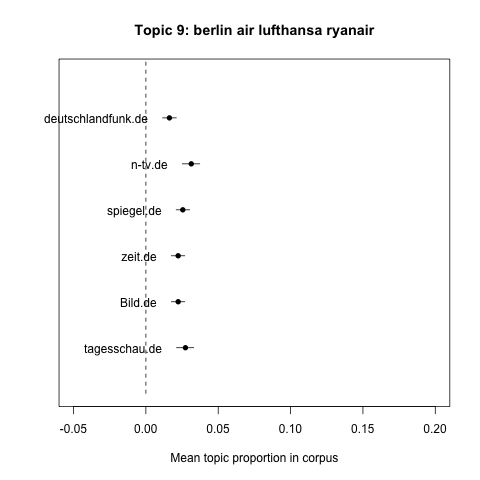
\includegraphics[width=\textwidth]{../figs/estimate_effect9.png}
		\end{subfigure}
				\begin{subfigure}[normla]{0.3\textwidth}
			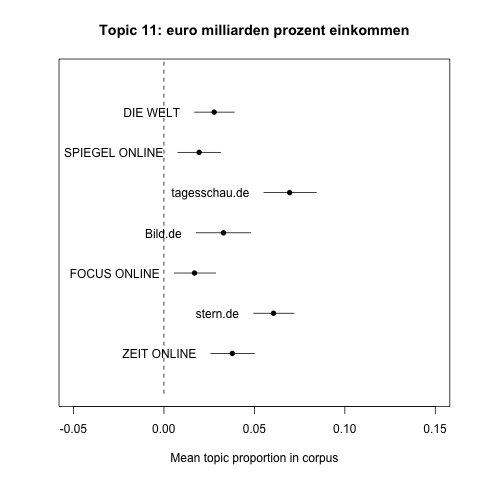
\includegraphics[width=\textwidth]{../figs/estimate_effect11.png}
		\end{subfigure}
				\begin{subfigure}[normla]{0.3\textwidth}
			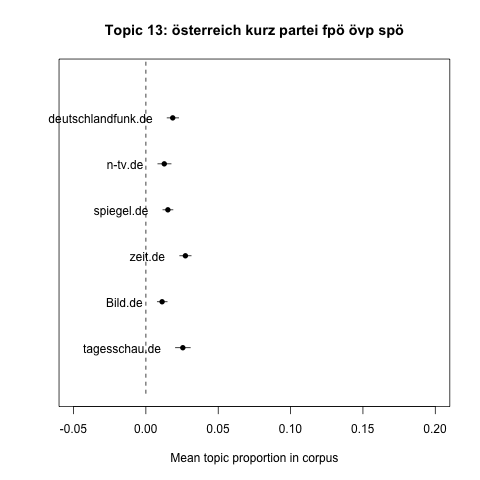
\includegraphics[width=\textwidth]{../figs/estimate_effect13.png}
		\end{subfigure}
				\begin{subfigure}[normla]{0.3\textwidth}
			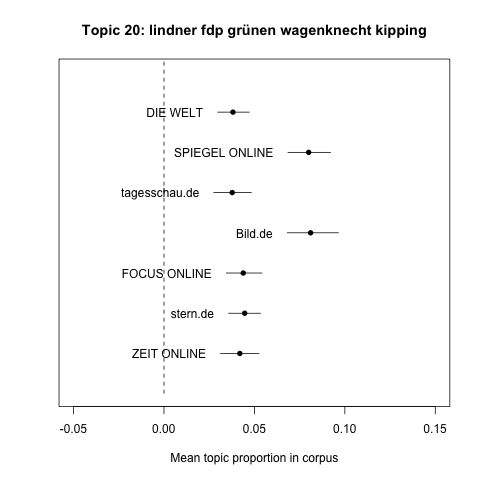
\includegraphics[width=\textwidth]{../figs/estimate_effect20.png}
		\end{subfigure}
				\begin{subfigure}[normla]{0.3\textwidth}
			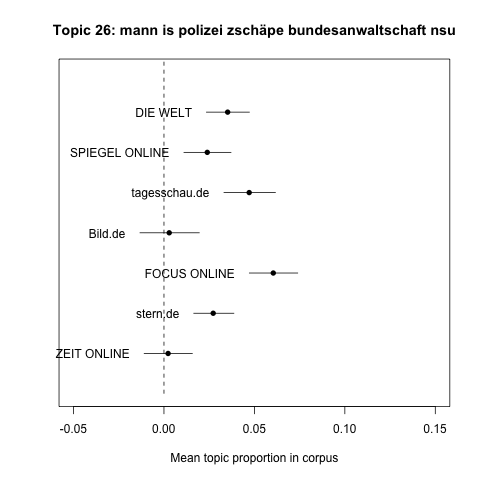
\includegraphics[width=\textwidth]{../figs/estimate_effect26.png}
		\end{subfigure}
	\end{center}
	\label{fig_estimateEffects_small}
\end{figure}

Another interesting aspect is how the news sources discusses the different topics, that is, describe the same event with different vocabulary.

\section{Distance Metric}

Since the topic distribution of a text is a simple mapping of text space, similarity of two texts can be measured by computing the topic distribution. KL distance is the measurement of “difference” between two probabilities. 

We use a probability distribution distance metric related to Jensen-Shannon divergence (JSD) to compare the word-topic distribution. Jensen-Shannon Divergence is a positive definite measure, satisfying the following conditions: $D_{js}(a,b) \geq 0$, $D_{js}(a,b)=0$ iff $(a=b)$. It is also symmetric: $D_{js}(a,b)=D_{js}(b,a)$. Let $p(x)$ and $q(x)$ be two probability density functions, the Jensen-Shannon distance $D_{js}(p,q)$ between this two distributions is defined as:

\begin{align*}
	D_{js}(p,q)=\frac{1}{2}D_{KL}(p,\frac{p+q}{2})+\frac{1}{2}D_{KL}(q,\frac{p+q}{2})
\end{align*}

where $D_{KL}$ is the Kullback-Leibler divergence between $p$ and $q$ defined as:

\begin{align*}
	D_{KL}(p,q)=\sum_{i=1}^T p_i ln \frac{p_i}{q_i}
\end{align*}

Since $D_{js}$ does not satisfy the triangular inequality condition $D_{js}(a,c)\leq D_{js}(a,c)+D_{js}(b,c)$, the JSD is not considered to be a real metric. On the other hand, the square root of JSD is a real distance metric \citep{endres_new_2003}. This is the reason why we use the square root and not JSD itself. 

\section{Sentiment analysis}

The idea of Sentiment analysis is to determine the attitude of a writer through online text data toward certain topic or the overall tonality of a document.

commonly used lexical or “bag-ofwords” approach. In that approach, the researcher provides pre-defined dictionaries (lists) of words associated with a given emotion, such as negativity. The target text is then deconstructed into individual words (or tokens) and the frequencies of words contained in a given dictionary are then calculated. For example, Loughran and McDonald (2011) construct a dictionary of words that express negativity in financial contexts, which they then use to measure the negativity in company 10-K filings and relate that negativity to financial outcomes.

The psychology literature demonstrates that any emotion can be parsimoniously defined by assigning it a score along two primary dimensions: valence (i.e., positive or negative) and arousal (i.e., activation and deactivation). For comparison purposes, we also examine three additional measures: “worried,” “satisfied,” and a lexical “negativity” measure. 

% ----------------------
% Appendix
% ----------------------
\section*{Appendix}

\begin{figure}[H]
	\caption{Mean prevalence of topics within each news source corpus 1}
	\begin{center}
		\begin{subfigure}[normla]{0.2\textwidth}
			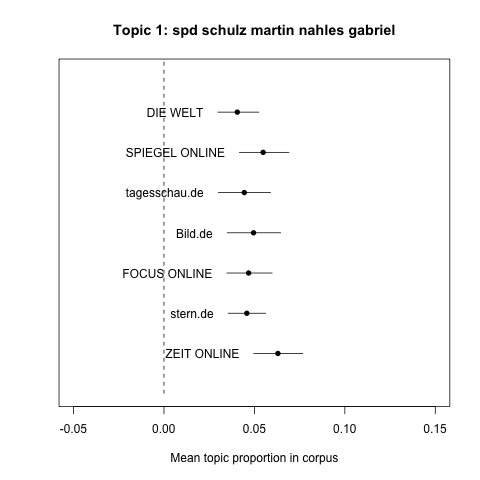
\includegraphics[width=\textwidth]{../figs/estimate_effect1.png}
		\end{subfigure}
		\begin{subfigure}[normla]{0.2\textwidth}
			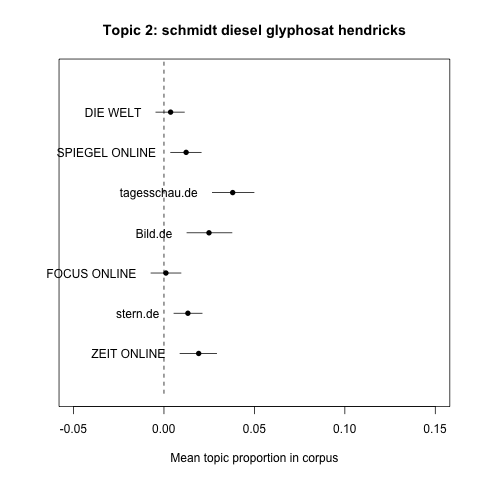
\includegraphics[width=\textwidth]{../figs/estimate_effect2.png}
		\end{subfigure}
				\begin{subfigure}[normla]{0.2\textwidth}
			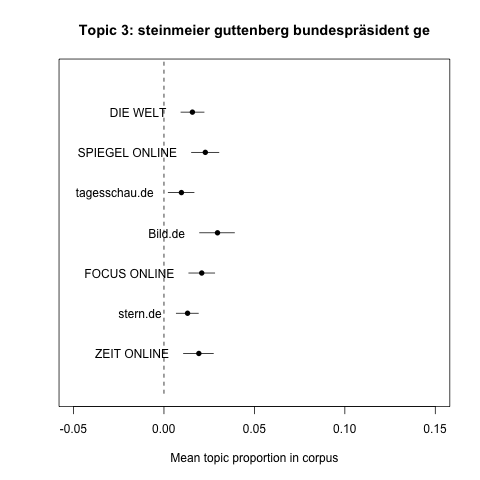
\includegraphics[width=\textwidth]{../figs/estimate_effect3.png}
		\end{subfigure}
				\begin{subfigure}[normla]{0.2\textwidth}
			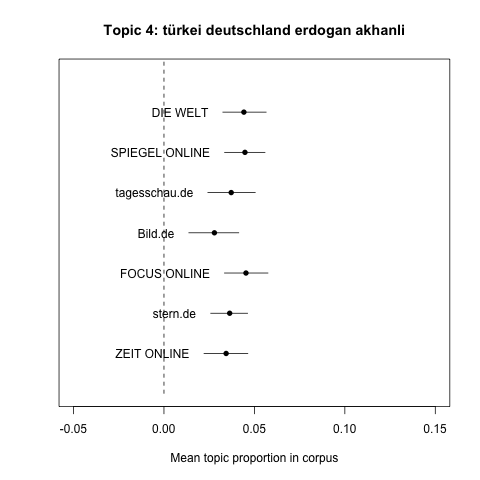
\includegraphics[width=\textwidth]{../figs/estimate_effect4.png}
		\end{subfigure}
				\begin{subfigure}[normla]{0.2\textwidth}
			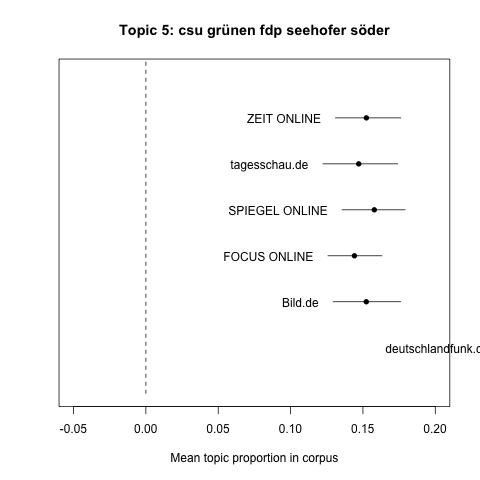
\includegraphics[width=\textwidth]{../figs/estimate_effect5.png}
		\end{subfigure}
				\begin{subfigure}[normla]{0.2\textwidth}
			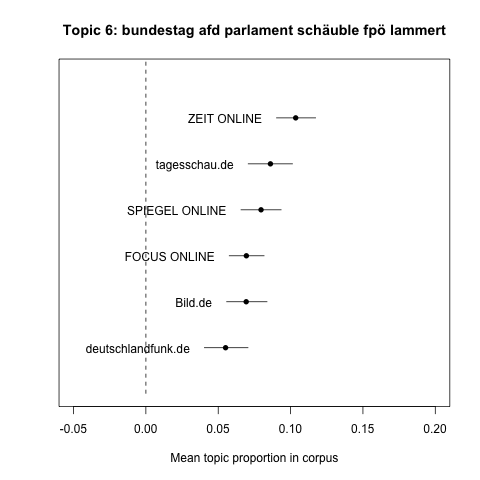
\includegraphics[width=\textwidth]{../figs/estimate_effect6.png}
		\end{subfigure}
		\begin{subfigure}[normla]{0.2\textwidth}
			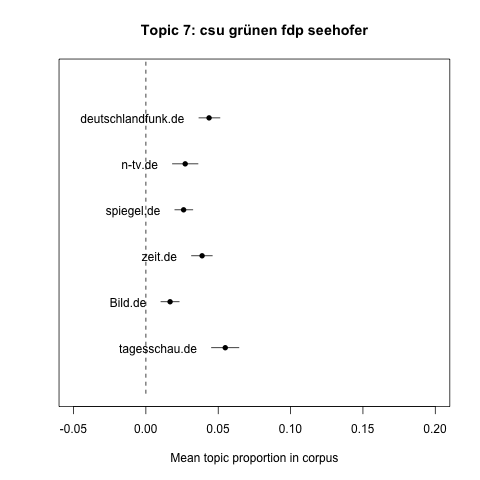
\includegraphics[width=\textwidth]{../figs/estimate_effect7.png}
		\end{subfigure}
		\begin{subfigure}[normla]{0.2\textwidth}
			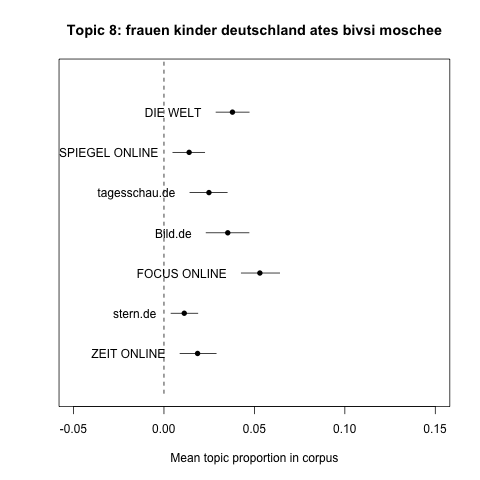
\includegraphics[width=\textwidth]{../figs/estimate_effect8.png}
		\end{subfigure}
		\begin{subfigure}[normla]{0.2\textwidth}
			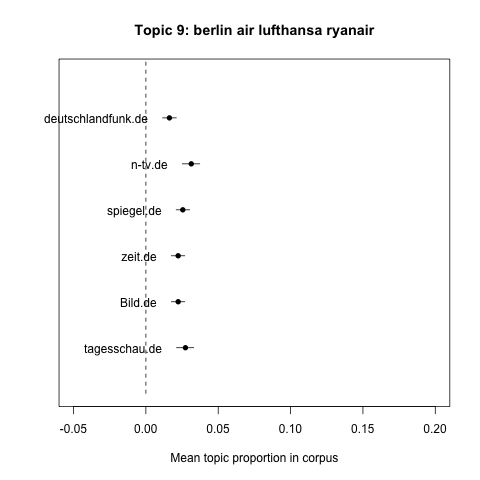
\includegraphics[width=\textwidth]{../figs/estimate_effect9.png}
		\end{subfigure}
		\begin{subfigure}[normla]{0.2\textwidth}
			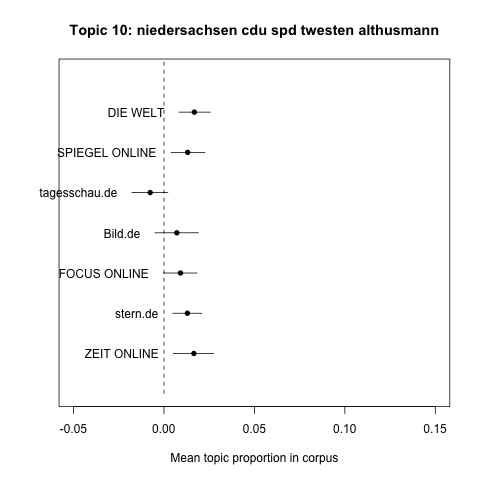
\includegraphics[width=\textwidth]{../figs/estimate_effect10.png}
		\end{subfigure}
		\begin{subfigure}[normla]{0.2\textwidth}
			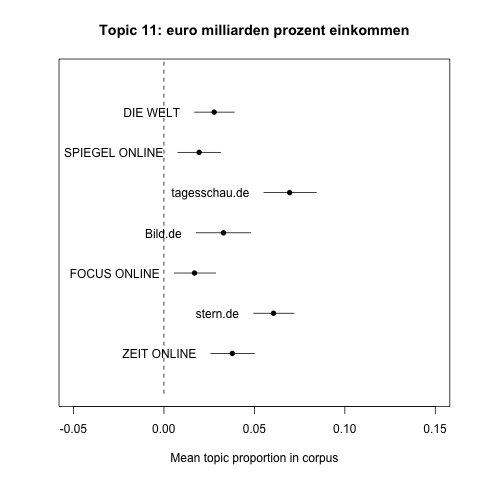
\includegraphics[width=\textwidth]{../figs/estimate_effect11.png}
		\end{subfigure}
		\begin{subfigure}[normla]{0.2\textwidth}
			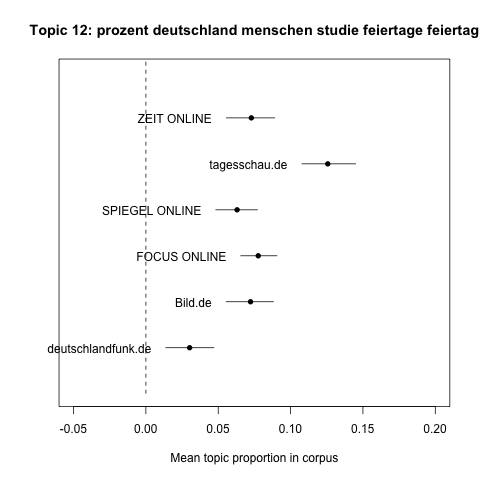
\includegraphics[width=\textwidth]{../figs/estimate_effect12.png}
		\end{subfigure}
		\begin{subfigure}[normla]{0.2\textwidth}
			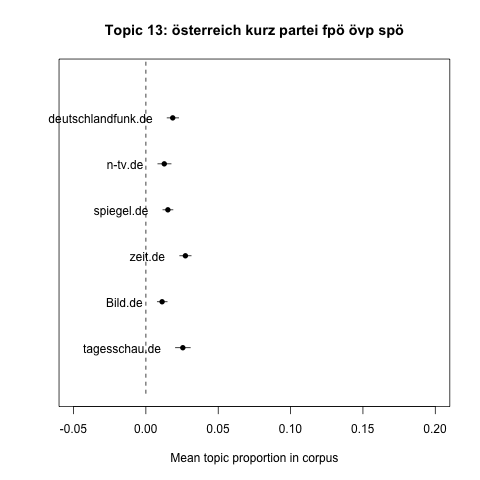
\includegraphics[width=\textwidth]{../figs/estimate_effect13.png}
		\end{subfigure}
		\begin{subfigure}[normla]{0.2\textwidth}
			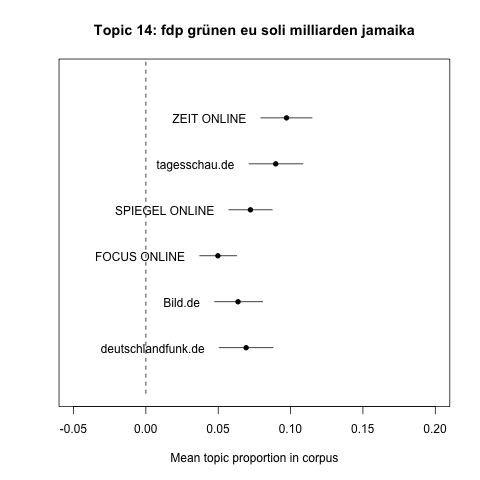
\includegraphics[width=\textwidth]{../figs/estimate_effect14.png}
		\end{subfigure}
	\end{center}
	\label{fig_estimateEffects_full1}
\end{figure}

\begin{figure}[H]
	\caption{Mean prevalence of topics within each news source corpus 2}
	\begin{center}
			\begin{subfigure}[normla]{0.2\textwidth}
			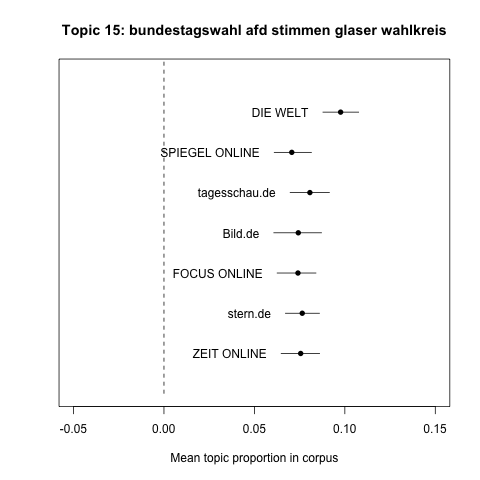
\includegraphics[width=\textwidth]{../figs/estimate_effect15.png}
		\end{subfigure}
		\begin{subfigure}[normla]{0.2\textwidth}
			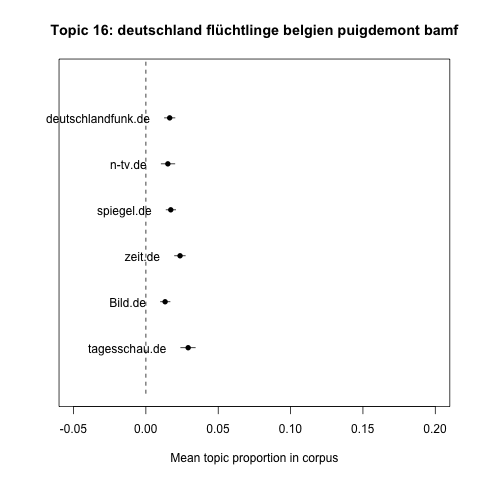
\includegraphics[width=\textwidth]{../figs/estimate_effect16.png}
		\end{subfigure}
		\begin{subfigure}[normla]{0.2\textwidth}
			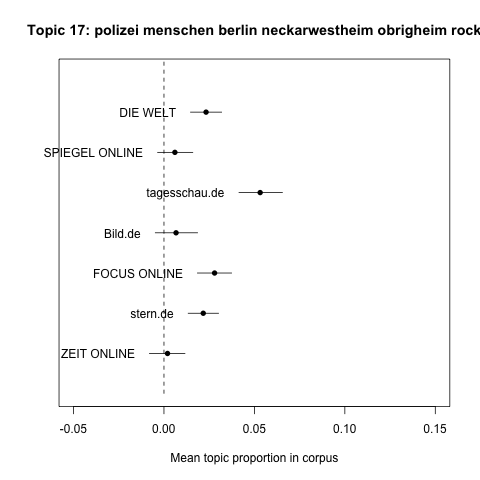
\includegraphics[width=\textwidth]{../figs/estimate_effect17.png}
		\end{subfigure}
		\begin{subfigure}[normla]{0.2\textwidth}
			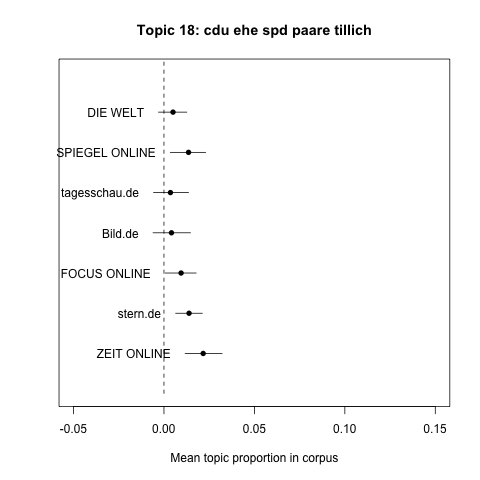
\includegraphics[width=\textwidth]{../figs/estimate_effect18.png}
		\end{subfigure}
		\begin{subfigure}[normla]{0.2\textwidth}
			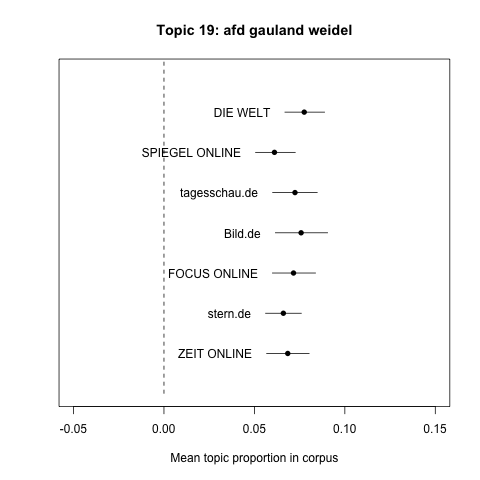
\includegraphics[width=\textwidth]{../figs/estimate_effect19.png}
		\end{subfigure}
		\begin{subfigure}[normla]{0.2\textwidth}
			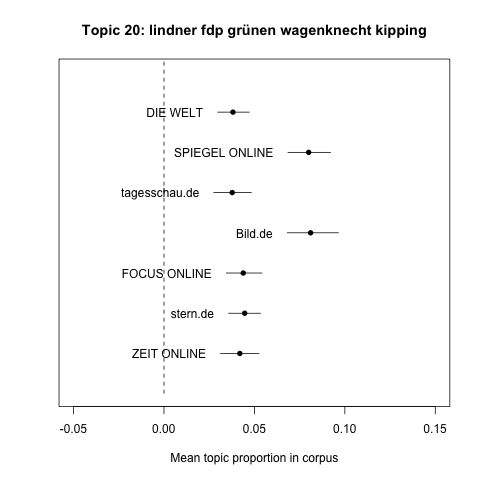
\includegraphics[width=\textwidth]{../figs/estimate_effect20.png}
		\end{subfigure}
		\begin{subfigure}[normla]{0.2\textwidth}
			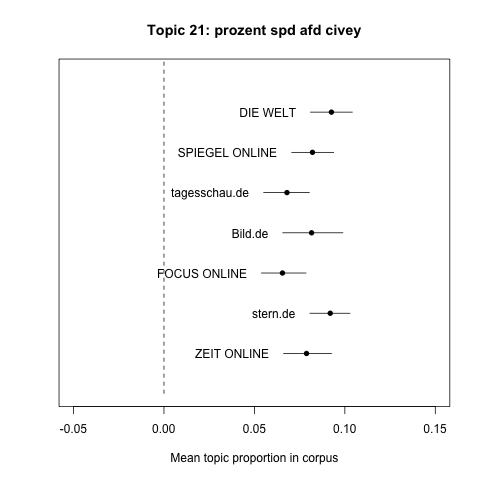
\includegraphics[width=\textwidth]{../figs/estimate_effect21.png}
		\end{subfigure}
		\begin{subfigure}[normla]{0.2\textwidth}
			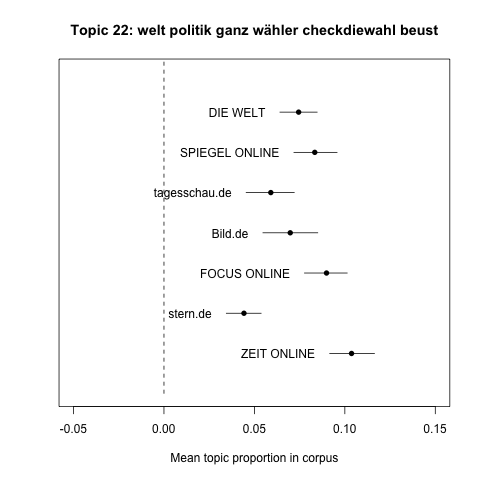
\includegraphics[width=\textwidth]{../figs/estimate_effect22.png}
		\end{subfigure}
		\begin{subfigure}[normla]{0.2\textwidth}
			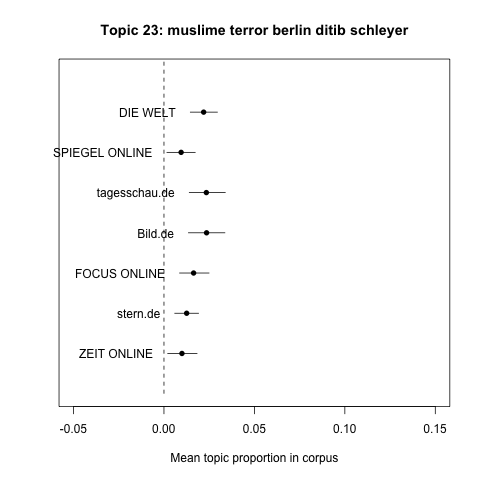
\includegraphics[width=\textwidth]{../figs/estimate_effect23.png}
		\end{subfigure}
		\begin{subfigure}[normla]{0.2\textwidth}
			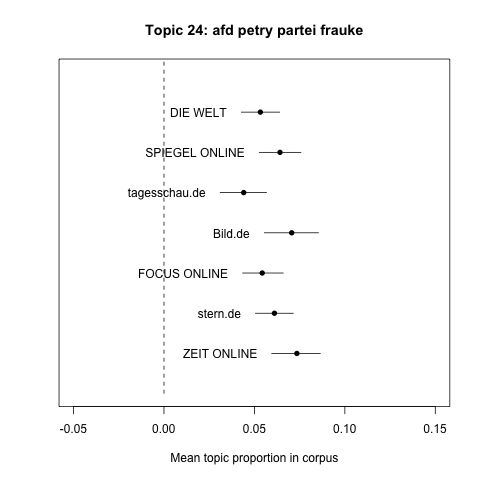
\includegraphics[width=\textwidth]{../figs/estimate_effect24.png}
		\end{subfigure}
		\begin{subfigure}[normla]{0.2\textwidth}
			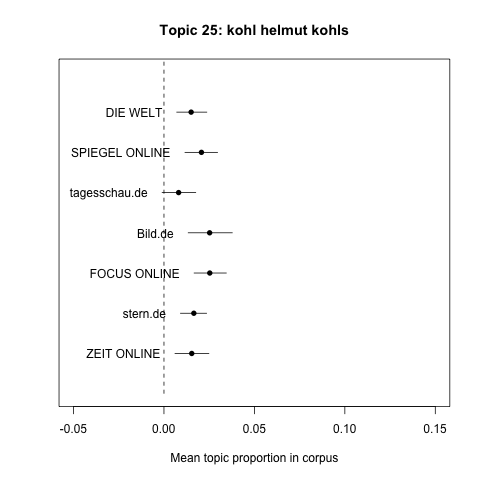
\includegraphics[width=\textwidth]{../figs/estimate_effect25.png}
		\end{subfigure}
		\begin{subfigure}[normla]{0.2\textwidth}
			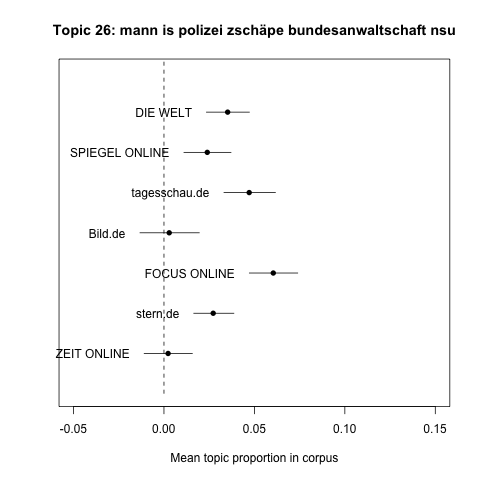
\includegraphics[width=\textwidth]{../figs/estimate_effect26.png}
		\end{subfigure}
				\begin{subfigure}[normla]{0.2\textwidth}
			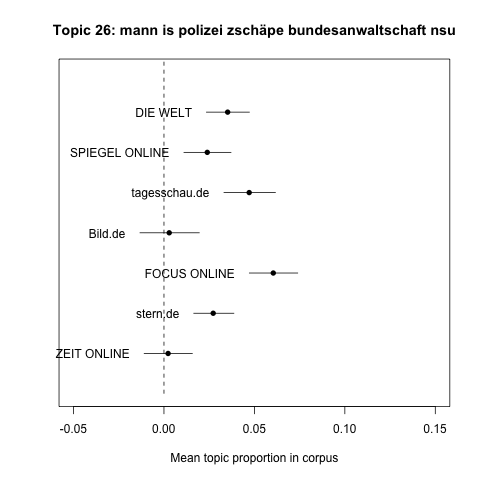
\includegraphics[width=\textwidth]{../figs/estimate_effect26.png}
		\end{subfigure}
				\begin{subfigure}[normla]{0.2\textwidth}
			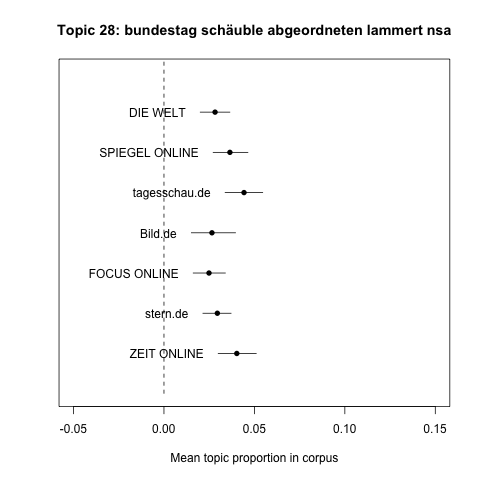
\includegraphics[width=\textwidth]{../figs/estimate_effect28.png}
		\end{subfigure}
	\end{center}
	\label{fig_estimateEffects_full2}
\end{figure}

\end{document}
